\chapter{Extensión No Lineal: Computación de Reservorio Estructurado}
\label{cap:sec_ssrc}

% --- SECCIÓN: Introducción y Motivación ---
\section{Introducción y Motivación}
\label{sec:ssrc_intro}
% ===================================================================

La sección precedente demostró que el marco TCROC-Markov logra
identificar regímenes económicos interpretables y produce pronósticos
estadísticamente superiores a los benchmarks evaluados.  Sin embargo,
la arquitectura subyacente es inherentemente \textbf{lineal}: el
operador $\alpha_t$ es un estimador de mínimos cuadrados ponderados, la discretización
K-Means opera sobre el espacio unidimensional de $\alpha_t$, y la
cadena de Markov de primer orden modela transiciones lineales entre
estados discretos.  Esta linealidad, si bien garantiza
interpretabilidad y estabilidad numérica, limita la capacidad del
marco para capturar dependencias no lineales en la dinámica de
precios.

El presente capítulo desarrolla una extensión que preserva la
estructura de estimación NNLS ya demostrada en los capítulos
anteriores, al tiempo que introduce capacidad de aproximación no
lineal mediante \textbf{Computación de Reservorio}
(\textit{Reservoir Computing}, RC) \cite{jaeger2001echo,
lukosevicius2009reservoir}.  La idea central es elegante en su
simplicidad: en lugar de alimentar directamente la señal $\alpha_t$
a un modelo de transición lineal, se la proyecta primero a un
espacio de alta dimensión mediante una transformación no lineal fija
(el \textit{reservorio}), y luego se estima la capa de lectura
mediante el \emph{mismo} procedimiento NNLS desarrollado en
secciones previas.

La contribución específica de este capítulo es quíntuple:
\begin{enumerate}
    \item La \textbf{formalización del Computador de Reservorio
    Estructurado Estocástico} (SSRC, \textit{Stochastically
    Structured Reservoir Computer}) \cite{banegas2025} como operador
    sobre espacios de señales, incluyendo la variante Leaky-ESN con
    factor de integración.
    \item La \textbf{demostración formal} de que el marco
    TCROC-Markov del capítulo anterior es un caso particular
    (degenerado) del SSRC, estableciendo una jerarquía de modelos.
    \item La \textbf{verificación de las condiciones} bajo las cuales
    la capa de lectura NNLS hereda las propiedades de existencia y
    unicidad ya establecidas.
    \item Un \textbf{análisis de estabilidad} del pronóstico bajo
    perturbaciones, con evaluación empírica de las cotas teóricas.
    \item Una \textbf{validación empírica comparativa} sobre los
    mismos datos de combustibles del
    Capítulo~\ref{cap:regimenes_combustibles}, incluyendo el
    test de Diebold-Mariano para significancia estadística.
\end{enumerate}

El estudio utiliza las mismas cuatro series semanales de precios de
combustibles en Honduras (Súper, Regular, Diésel y Kerosene) y el
mismo protocolo de ventanas deslizantes del capítulo anterior, con
conjunto de entrenamiento inicial de 312 semanas (enero 2017 --
diciembre 2022) y horizonte de pronóstico de 1 semana, para garantizar
la comparabilidad estricta de los resultados.

% --- SECCIÓN: Marco Teórico del Computador de Reservorio ---
\section{Marco Teórico del Computador de Reservorio}
\label{sec:ssrc_marco_teorico}

% --- SUBSECCIÓN: Sistemas Dinámicos con Entrada --- - - - - - - - - - - - - - - - - - - - - - - - - - - - - - -
\subsection{Sistemas Dinámicos con Entrada}
\label{subsec:sistemas_dinamicos_entrada}
% -------------------------------------------------------------------

Comenzamos situando la computación de reservorio dentro del marco
general de los sistemas dinámicos discretos con entrada.

\begin{definition}[Sistema dinámico con entrada]
\label{def:sistema_dinamico_entrada}
Sean $\set{U} \subseteq \mathbb{R}^d$ el espacio de entradas,
$\set{H} \subseteq \mathbb{R}^D$ el espacio de estados internos, y
$\set{Y} \subseteq \mathbb{R}^m$ el espacio de salidas.  Un
\textbf{sistema dinámico discreto con entrada} es una tripleta
$(\set{U}, F, G)$ donde
\begin{align}
    F &: \set{H} \times \set{U} \to \set{H}, \label{eq:mapa_estado}\\
    G &: \set{H} \to \set{Y}, \label{eq:mapa_lectura}
\end{align}
de modo que la evolución del sistema se rige por
\begin{equation}
    \vect{h}_t = F(\vect{h}_{t-1}, \vect{u}_t), \qquad
    \vect{y}_t = G(\vect{h}_t),
    \label{eq:evolucion_general}
\end{equation}
para $t = 1, 2, \ldots$, con condición inicial
$\vect{h}_0 \in \set{H}$.
\end{definition}

En este marco, la \emph{computación} consiste en aprender el mapa
de lectura $G$ a partir de datos observados, manteniendo el mapa de
estado $F$ fijo.  Esta separación es la idea fundamental de la
computación de reservorio.

% --- SUBSECCIÓN: El Computador de Reservorio (Echo State Network) --- - - - - - - - - - - - - - - - - - - - - - - - - - - - - - -
\subsection{El Computador de Reservorio (Echo State Network)}
\label{subsec:esn_definicion}
% -------------------------------------------------------------------

\begin{definition}[Computador de Reservorio]
\label{def:computador_reservorio}
Un \textbf{Computador de Reservorio} (RC) de dimensión $D$ con
función de activación $\sigma: \mathbb{R} \to \mathbb{R}$ es un
sistema dinámico con entrada $(\set{U}, F_{\text{RC}}, G_{\text{RC}})$
donde:
\begin{enumerate}
    \item El mapa de estado tiene la forma
    \begin{equation}
        F_{\text{RC}}(\vect{h}, \vect{u}) =
        \sigma\!\left(\mat{W}_{\text{in}}\,\vect{u} +
        \mat{W}_{\text{res}}\,\vect{h}\right),
        \label{eq:mapa_estado_rc}
    \end{equation}
    con $\mat{W}_{\text{in}} \in \mathbb{R}^{D \times d}$ la
    \textbf{matriz de entrada},
    $\mat{W}_{\text{res}} \in \mathbb{R}^{D \times D}$ la
    \textbf{matriz de reservorio}, y $\sigma$ aplicada
    componente a componente.
    \item El mapa de lectura es lineal:
    \begin{equation}
        G_{\text{RC}}(\vect{h}) = \mat{W}_{\text{out}}\,\vect{h},
        \label{eq:mapa_lectura_rc}
    \end{equation}
    con $\mat{W}_{\text{out}} \in \mathbb{R}^{m \times D}$ la
    \textbf{matriz de lectura}.
    \item Las matrices $\mat{W}_{\text{in}}$ y
    $\mat{W}_{\text{res}}$ son \textbf{fijas} (no se optimizan);
    solo $\mat{W}_{\text{out}}$ se estima a partir de datos.
\end{enumerate}
\end{definition}

La ecuación de estado se expande recursivamente como
\begin{equation}
    \vect{h}_t = \sigma\!\left(\mat{W}_{\text{in}}\,\vect{u}_t +
    \mat{W}_{\text{res}}\,
    \sigma\!\left(\mat{W}_{\text{in}}\,\vect{u}_{t-1} +
    \mat{W}_{\text{res}}\,\vect{h}_{t-2}\right)\right),
    \label{eq:expansion_recursiva}
\end{equation}
lo que muestra que $\vect{h}_t$ es una función no lineal de toda la
historia de entradas $(\vect{u}_1, \ldots, \vect{u}_t)$ y de la
condición inicial $\vect{h}_0$.  El reservorio actúa como una
\textbf{memoria no lineal} que codifica el pasado de la señal en un
espacio de dimensión $D \gg d$.

% --- SUBSECCIÓN: Variante con Integración de Fuga (Leaky-ESN) --- - - - - - - - - - - - - - - - - - - - - - - - - - - - - - -
\subsection{Variante con Integración de Fuga (Leaky-ESN)}
\label{subsec:leaky_esn}
% -------------------------------------------------------------------

En aplicaciones donde la señal de entrada exhibe alta persistencia,
como ocurre en el caso del mercado regulado de combustibles hondureños
(Capítulo~\ref{cap:regimenes_combustibles}), resulta ventajoso
introducir un mecanismo de suavizado temporal explícito en la
ecuación de estado.

\begin{definition}[Computador de Reservorio con Integración de Fuga]
\label{def:leaky_esn}
Un \textbf{Leaky-ESN} \cite{jaeger2001echo} es un Computador de
Reservorio (Definición~\ref{def:computador_reservorio}) cuyo mapa
de estado se modifica como:
\begin{equation}
    \vect{h}_t = (1 - a)\,\vect{h}_{t-1} + a\,\sigma\!\left(
    \mat{W}_{\text{in}}\,\vect{u}_t +
    \mat{W}_{\text{res}}\,\vect{h}_{t-1}\right),
    \label{eq:leaky_esn}
\end{equation}
donde $a \in (0, 1]$ es el \textbf{factor de fuga}
(\textit{leak rate}).  El caso $a = 1$ recupera la ESN estándar
de la Definición~\ref{def:computador_reservorio}.
\end{definition}

El parámetro $a$ controla la \emph{escala temporal efectiva} del
reservorio.  Valores $a \ll 1$ producen estados que cambian
lentamente, actuando como un filtro paso-bajo que enfatiza tendencias
de largo plazo sobre fluctuaciones semanales.  Formalmente, la
ecuación~\eqref{eq:leaky_esn} puede interpretarse como la
discretización de Euler de un sistema dinámico continuo con constante
de tiempo $\tau = 1/a$, de modo que $a = 0.1$ corresponde a
$\tau = 10$ pasos temporales de memoria efectiva.

\begin{remark}[Preservación de la ESP para Leaky-ESN]
\label{obs:esp_leaky}
La variante Leaky-ESN preserva la ESP bajo la misma condición
$\rho(\mat{W}_{\text{res}}) < 1$ del Teorema~\ref{teo:esp_suficiente}.
La demostración es análoga: la mezcla convexa
$(1-a)\vect{h}_{t-1} + a\,\sigma(\cdot)$ mantiene la contractibilidad
pues $(1-a) + a \cdot \|\mat{W}_{\text{res}}\| < 1$ cuando
$\|\mat{W}_{\text{res}}\| < 1$.
\end{remark}

% --- SUBSECCIÓN: El Computador de Reservorio Estructurado Estocástico (SSRC) --- - - - - - - - - - - - - - - - - - - - - - - - - - - - - - -
\subsection{El Computador de Reservorio Estructurado Estocástico (SSRC)}
\label{subsec:ssrc_definicion}
% -------------------------------------------------------------------

\begin{definition}[Computador de Reservorio Estructurado Estocástico
(SSRC)]
\label{def:ssrc}
Un \textbf{SSRC} \cite{banegas2025} es un Computador de Reservorio
con Integración de Fuga
(Definición~\ref{def:leaky_esn}) con las siguientes
especializaciones:
\begin{enumerate}
    \item La función de activación es $\sigma = \tanh$.
    \item La matriz de entrada $\mat{W}_{\text{in}}$ se genera
    aleatoriamente con entradas i.i.d.\ de una distribución
    uniforme en $[-\omega, \omega]$ para algún $\omega > 0$.
    \item La matriz de reservorio $\mat{W}_{\text{res}}$ se genera
    como una matriz dispersa aleatoria y se reescala a un radio
    espectral objetivo $\rho_{\text{res}}$:
    \begin{equation}
        \mat{W}_{\text{res}} \leftarrow
        \rho_{\text{res}} \cdot
        \frac{\mat{W}_{\text{res}}^{(0)}}
        {\rho(\mat{W}_{\text{res}}^{(0)})},
        \label{eq:reescalado_espectral}
    \end{equation}
    donde $\mat{W}_{\text{res}}^{(0)}$ es la matriz dispersa
    inicial y $\rho(\cdot)$ denota el radio espectral.
    \item La matriz de lectura $\mat{W}_{\text{out}}$ se estima
    mediante NNLS.
\end{enumerate}
Los hiperparámetros del SSRC son la tripleta
$(D, \rho_{\text{res}}, a)$: dimensión, radio espectral y factor
de fuga, respectivamente.
\end{definition}

% --- SUBSECCIÓN: La Propiedad de Estado de Eco --- - - - - - - - - - - - - - - - - - - - - - - - - - - - - - -
\subsection{La Propiedad de Estado de Eco}
\label{subsec:echo_state_property}
% -------------------------------------------------------------------

La utilidad práctica de un computador de reservorio depende de que la
influencia de la condición inicial $\vect{h}_0$ se desvanezca
asintóticamente, de modo que la salida dependa únicamente de la
secuencia de entradas.  Esta condición se formaliza a continuación.

\begin{definition}[Propiedad de Estado de Eco (ESP)]
\label{def:esp}
Sea $(\set{U}, F_{\text{RC}}, G_{\text{RC}})$ un Computador de
Reservorio.  Se dice que posee la \textbf{Propiedad de Estado de Eco}
(ESP) si, para toda secuencia de entradas acotada
$\{\vect{u}_t\}_{t \in \mathbb{Z}} \subset \set{U}$, existe una
única secuencia de estados $\{\vect{h}_t\}_{t \in \mathbb{Z}}
\subset \set{H}$ compatible con~\eqref{eq:mapa_estado_rc}, y esta
secuencia es independiente de la condición inicial.  Formalmente,
para cualesquiera $\vect{h}_0, \vect{h}_0' \in \set{H}$:
\begin{equation}
    \lim_{t \to \infty} \left\|
    F^{(t)}(\vect{h}_0, \vect{u}_{1:t}) -
    F^{(t)}(\vect{h}_0', \vect{u}_{1:t})
    \right\| = 0,
    \label{eq:esp_formal}
\end{equation}
donde $F^{(t)}$ denota la composición $t$-ésima del mapa de estado.
\end{definition}

\begin{theorem}[Condición suficiente para la ESP]
\label{teo:esp_suficiente}
Sea $(\set{U}, F_{\text{RC}}, G_{\text{RC}})$ un Computador de
Reservorio con $\sigma = \tanh$ y entradas acotadas
$\|\vect{u}_t\| \le U_{\max}$ para todo $t$.  Si
\begin{equation}
    \rho(\mat{W}_{\text{res}}) < 1,
    \label{eq:condicion_esp}
\end{equation}
entonces el sistema posee la ESP.
\end{theorem}

\begin{proof}
Consideremos dos trayectorias $\{\vect{h}_t\}$ y
$\{\vect{h}_t'\}$ generadas por la misma secuencia de entradas
pero con condiciones iniciales distintas $\vect{h}_0 \ne
\vect{h}_0'$.  Para $t \ge 1$:
\begin{align}
    \vect{h}_t - \vect{h}_t' &=
    \sigma(\mat{W}_{\text{in}}\vect{u}_t +
    \mat{W}_{\text{res}}\vect{h}_{t-1}) -
    \sigma(\mat{W}_{\text{in}}\vect{u}_t +
    \mat{W}_{\text{res}}\vect{h}_{t-1}').
    \label{eq:diferencia_trayectorias}
\end{align}
Dado que $\tanh$ es Lipschitz continua con constante $L = 1$
(pues $|\tanh'(x)| = 1 - \tanh^2(x) \le 1$ para todo
$x \in \mathbb{R}$), se tiene componente a componente:
\begin{equation}
    \|\vect{h}_t - \vect{h}_t'\| \le
    \|\mat{W}_{\text{res}}(\vect{h}_{t-1} - \vect{h}_{t-1}')\|
    \le \|\mat{W}_{\text{res}}\|\,
    \|\vect{h}_{t-1} - \vect{h}_{t-1}'\|,
    \label{eq:contraccion_paso}
\end{equation}
donde $\|\mat{W}_{\text{res}}\|$ denota la norma espectral
(mayor valor singular).  Aplicando inductivamente:
\begin{equation}
    \|\vect{h}_t - \vect{h}_t'\| \le
    \|\mat{W}_{\text{res}}\|^t\,
    \|\vect{h}_0 - \vect{h}_0'\|.
    \label{eq:contraccion_inductiva}
\end{equation}
Por la fórmula de Gelfand, $\rho(\mat{W}_{\text{res}}) =
\lim_{n \to \infty} \|\mat{W}_{\text{res}}^n\|^{1/n}$, de modo
que la condición $\rho(\mat{W}_{\text{res}}) < 1$ implica la
existencia de $n_0 \in \mathbb{N}$ y $\delta \in (0,1)$ tales que
$\|\mat{W}_{\text{res}}^n\| \le \delta^n$ para todo $n \ge n_0$.
Reagrupando la iteración en bloques de tamaño $n_0$:
\begin{equation}
    \|\vect{h}_{kn_0} - \vect{h}_{kn_0}'\| \le
    \delta^k\, C\, \|\vect{h}_0 - \vect{h}_0'\|,
    \label{eq:contraccion_gelfand}
\end{equation}
donde $C = \max_{0 \le j < n_0} \|\mat{W}_{\text{res}}^j\|$.
Como $\delta < 1$, el lado derecho converge a cero
exponencialmente conforme $k \to \infty$, lo que
establece~\eqref{eq:esp_formal}.
\end{proof}

\begin{remark}[Sobre la condición $\rho < 1$]
\label{obs:rho_condicion}
La condición $\rho(\mat{W}_{\text{res}}) < 1$ es suficiente
pero no necesaria para la ESP.  Yildiz et al.\ \cite{yildiz2012}
mostraron que la ESP puede sostenerse incluso con
$\rho(\mat{W}_{\text{res}}) > 1$ para ciertas clases de entradas.
No obstante, la condición $\rho < 1$ es verificable a priori y
se impone constructivamente mediante el
reescalado~\eqref{eq:reescalado_espectral}, por lo que constituye
la condición estándar en implementaciones prácticas.
\end{remark}

% --- SUBSECCIÓN: Capacidad de Aproximación Universal --- - - - - - - - - - - - - - - - - - - - - - - - - - - - - - -
\subsection{Capacidad de Aproximación Universal}
\label{subsec:aproximacion_universal}
% -------------------------------------------------------------------

La justificación teórica para utilizar un reservorio como extractor
de características proviene del siguiente resultado fundamental.

\begin{theorem}[Aproximación universal por reservorios
{\cite[Teorema~3.1]{grigoryeva2018universal}}]
\label{teo:aproximacion_universal}
Sean $\set{U} \subset \mathbb{R}^d$ compacto y $\set{F}$ el
conjunto de funcionales causales e invariantes en el tiempo
$H: \set{U}^{\mathbb{Z}_{-}} \to \mathbb{R}^m$ que son continuos
respecto a la topología del producto.  Para todo $H \in \set{F}$ y
todo $\varepsilon > 0$, existen un Computador de Reservorio con
la ESP de dimensión $D$ suficientemente grande y una matriz de
lectura $\mat{W}_{\text{out}} \in \mathbb{R}^{m \times D}$ tales
que
\begin{equation}
    \sup_{\{\vect{u}_t\} \in \set{U}^{\mathbb{Z}_{-}}}
    \|H(\ldots, \vect{u}_{t-1}, \vect{u}_t) -
    \mat{W}_{\text{out}}\,\vect{h}_t\| < \varepsilon.
    \label{eq:aproximacion_universal}
\end{equation}
\end{theorem}

Este resultado establece que los computadores de reservorio con la
ESP son \textbf{aproximadores universales de funcionales sobre
secuencias}.  A diferencia de los teoremas de aproximación universal
para redes neuronales feedforward (que aproximan funciones estáticas),
el Teorema~\ref{teo:aproximacion_universal} garantiza la aproximación
de mapas \emph{con memoria}: funciones que dependen de toda la
historia pasada de la señal.  En nuestro contexto, esto significa que
un reservorio de dimensión suficiente puede, en principio, capturar
cualquier dependencia no lineal entre el historial de precios
$\{v_1, \ldots, v_t\}$ y el precio futuro $v_{t+1}$, siempre que
esta dependencia sea continua y causal.

% --- SECCIÓN: TCROC-Markov como Caso Particular del SSRC ---
\section{TCROC-Markov como Caso Particular del SSRC}
\label{sec:tcroc_como_caso_particular}
% ===================================================================

Esta sección establece el resultado central del capítulo: la
relación formal de inclusión entre el marco lineal del
Capítulo~\ref{cap:regimenes_combustibles} y el marco no lineal del
SSRC.

% --- SUBSECCIÓN: Reformulación del Marco Lineal --- - - - - - - - - - - - - - - - - - - - - - - - - - - - - - -
\subsection{Reformulación del Marco Lineal}
\label{subsec:reformulacion_lineal}
% -------------------------------------------------------------------

Para establecer la conexión, reformulamos el flujo de trabajo
TCROC-Markov como un caso de la
Definición~\ref{def:sistema_dinamico_entrada}.

\begin{definition}[Sistema TCROC-Markov como sistema dinámico]
\label{def:tcroc_como_sistema}
El marco TCROC-Markov con hiperparámetros $(W, \lambda, K)$ es un
sistema dinámico con entrada
$(\mathbb{R}, F_{\text{TM}}, G_{\text{TM}})$ donde:
\begin{enumerate}
    \item La entrada es $u_t = \alpha_t \in \mathbb{R}$.
    \item El espacio de estados es $\set{H}_{\text{TM}} =
    \{\vect{e}_1, \ldots, \vect{e}_K\} \subset \mathbb{R}^K$
    (los vectores canónicos).
    \item El mapa de estado es
    $F_{\text{TM}}(\vect{h}, u) = \vect{e}_{Q(u)}$, donde
    $Q: \mathbb{R} \to \{1, \ldots, K\}$ es la función de
    asignación K-Means.
    \item El mapa de lectura es
    $G_{\text{TM}}(\vect{h}) = \hat{\mat{P}}\,\vect{h}$,
    con $\hat{\mat{P}} \in \mathbb{R}^{K \times K}$ la matriz
    de transición estimada.
\end{enumerate}
\end{definition}

Observemos que en este sistema: (a) el mapa de estado $F_{\text{TM}}$
no tiene memoria interna (depende solo de $u_t$, no de
$\vect{h}_{t-1}$); (b) la no linealidad está contenida únicamente
en la cuantización $Q$; y (c) el mapa de lectura es estrictamente
lineal.

% --- SUBSECCIÓN: El Teorema de Inclusión --- - - - - - - - - - - - - - - - - - - - - - - - - - - - - - -
\subsection{El Teorema de Inclusión}
\label{subsec:teorema_inclusion}
% -------------------------------------------------------------------

\begin{theorem}[TCROC-Markov como reservorio degenerado]
\label{teo:inclusion}
Sea $(\set{U}, F_{\text{RC}}, G_{\text{RC}})$ un Computador de
Reservorio de dimensión $D = K$ con:
\begin{enumerate}
    \item[(i)] Matriz de reservorio nula:
    $\mat{W}_{\text{res}} = \mat{0}_{K \times K}$.
    \item[(ii)] Función de activación identidad:
    $\sigma = \mathrm{id}$.
    \item[(iii)] Matriz de entrada definida por la cuantización
    K-Means: $\mat{W}_{\text{in}} = [\vect{e}_{Q(\cdot)}]$,
    es decir, $F_{\text{RC}}(\vect{h}, u) = \vect{e}_{Q(u)}$.
    \item[(iv)] Matriz de lectura
    $\mat{W}_{\text{out}} = \hat{\mat{P}}$.
    \item[(v)] Factor de fuga $a = 1$ (ESN estándar).
\end{enumerate}
Entonces, para toda secuencia de entradas $\{u_t = \alpha_t\}$ y
toda condición inicial $\vect{h}_0$:
\begin{equation}
    G_{\text{RC}}(\vect{h}_t) = G_{\text{TM}}(\vect{h}_t) =
    \hat{\mat{P}}\,\vect{e}_{S_t} \qquad \forall\, t \ge 1.
    \label{eq:equivalencia_sistemas}
\end{equation}
Además, el sistema satisface trivialmente la ESP: la convergencia
en~\eqref{eq:esp_formal} es instantánea (en un solo paso).
\end{theorem}

\begin{proof}
\textbf{Equivalencia de salidas.}  Bajo las condiciones
(i)--(iii) y (v), el mapa de estado~\eqref{eq:leaky_esn} se
reduce a:
\begin{equation}
    \vect{h}_t = (1-1)\vect{h}_{t-1} + 1 \cdot \mathrm{id}\!\left(
    \mat{W}_{\text{in}}\,u_t + \mat{0}\cdot\vect{h}_{t-1}
    \right) = \vect{e}_{Q(u_t)} = \vect{e}_{S_t}.
\end{equation}
Con la condición (iv), la salida es
$G_{\text{RC}}(\vect{h}_t) =
\hat{\mat{P}}\,\vect{e}_{S_t}$, que coincide con
$G_{\text{TM}}$.

\textbf{ESP instantánea.}  Para cualesquiera
$\vect{h}_0, \vect{h}_0'$, a partir de $t = 1$:
$\vect{h}_1 = \vect{e}_{Q(u_1)} = \vect{h}_1'$,
independientemente de $\vect{h}_0$ y $\vect{h}_0'$.  Por tanto,
$\|\vect{h}_t - \vect{h}_t'\| = 0$ para todo $t \ge 1$.
\end{proof}

La Figura~\ref{fig:ssrc_inclusion} verifica numéricamente este
resultado: la diferencia máxima entre las salidas de TCROC-Markov
y del reservorio degenerado es exactamente $0.0$ para las cuatro
series, confirmando la identidad algebraica a nivel de precisión
de máquina.

\begin{figure}[H]
\centering
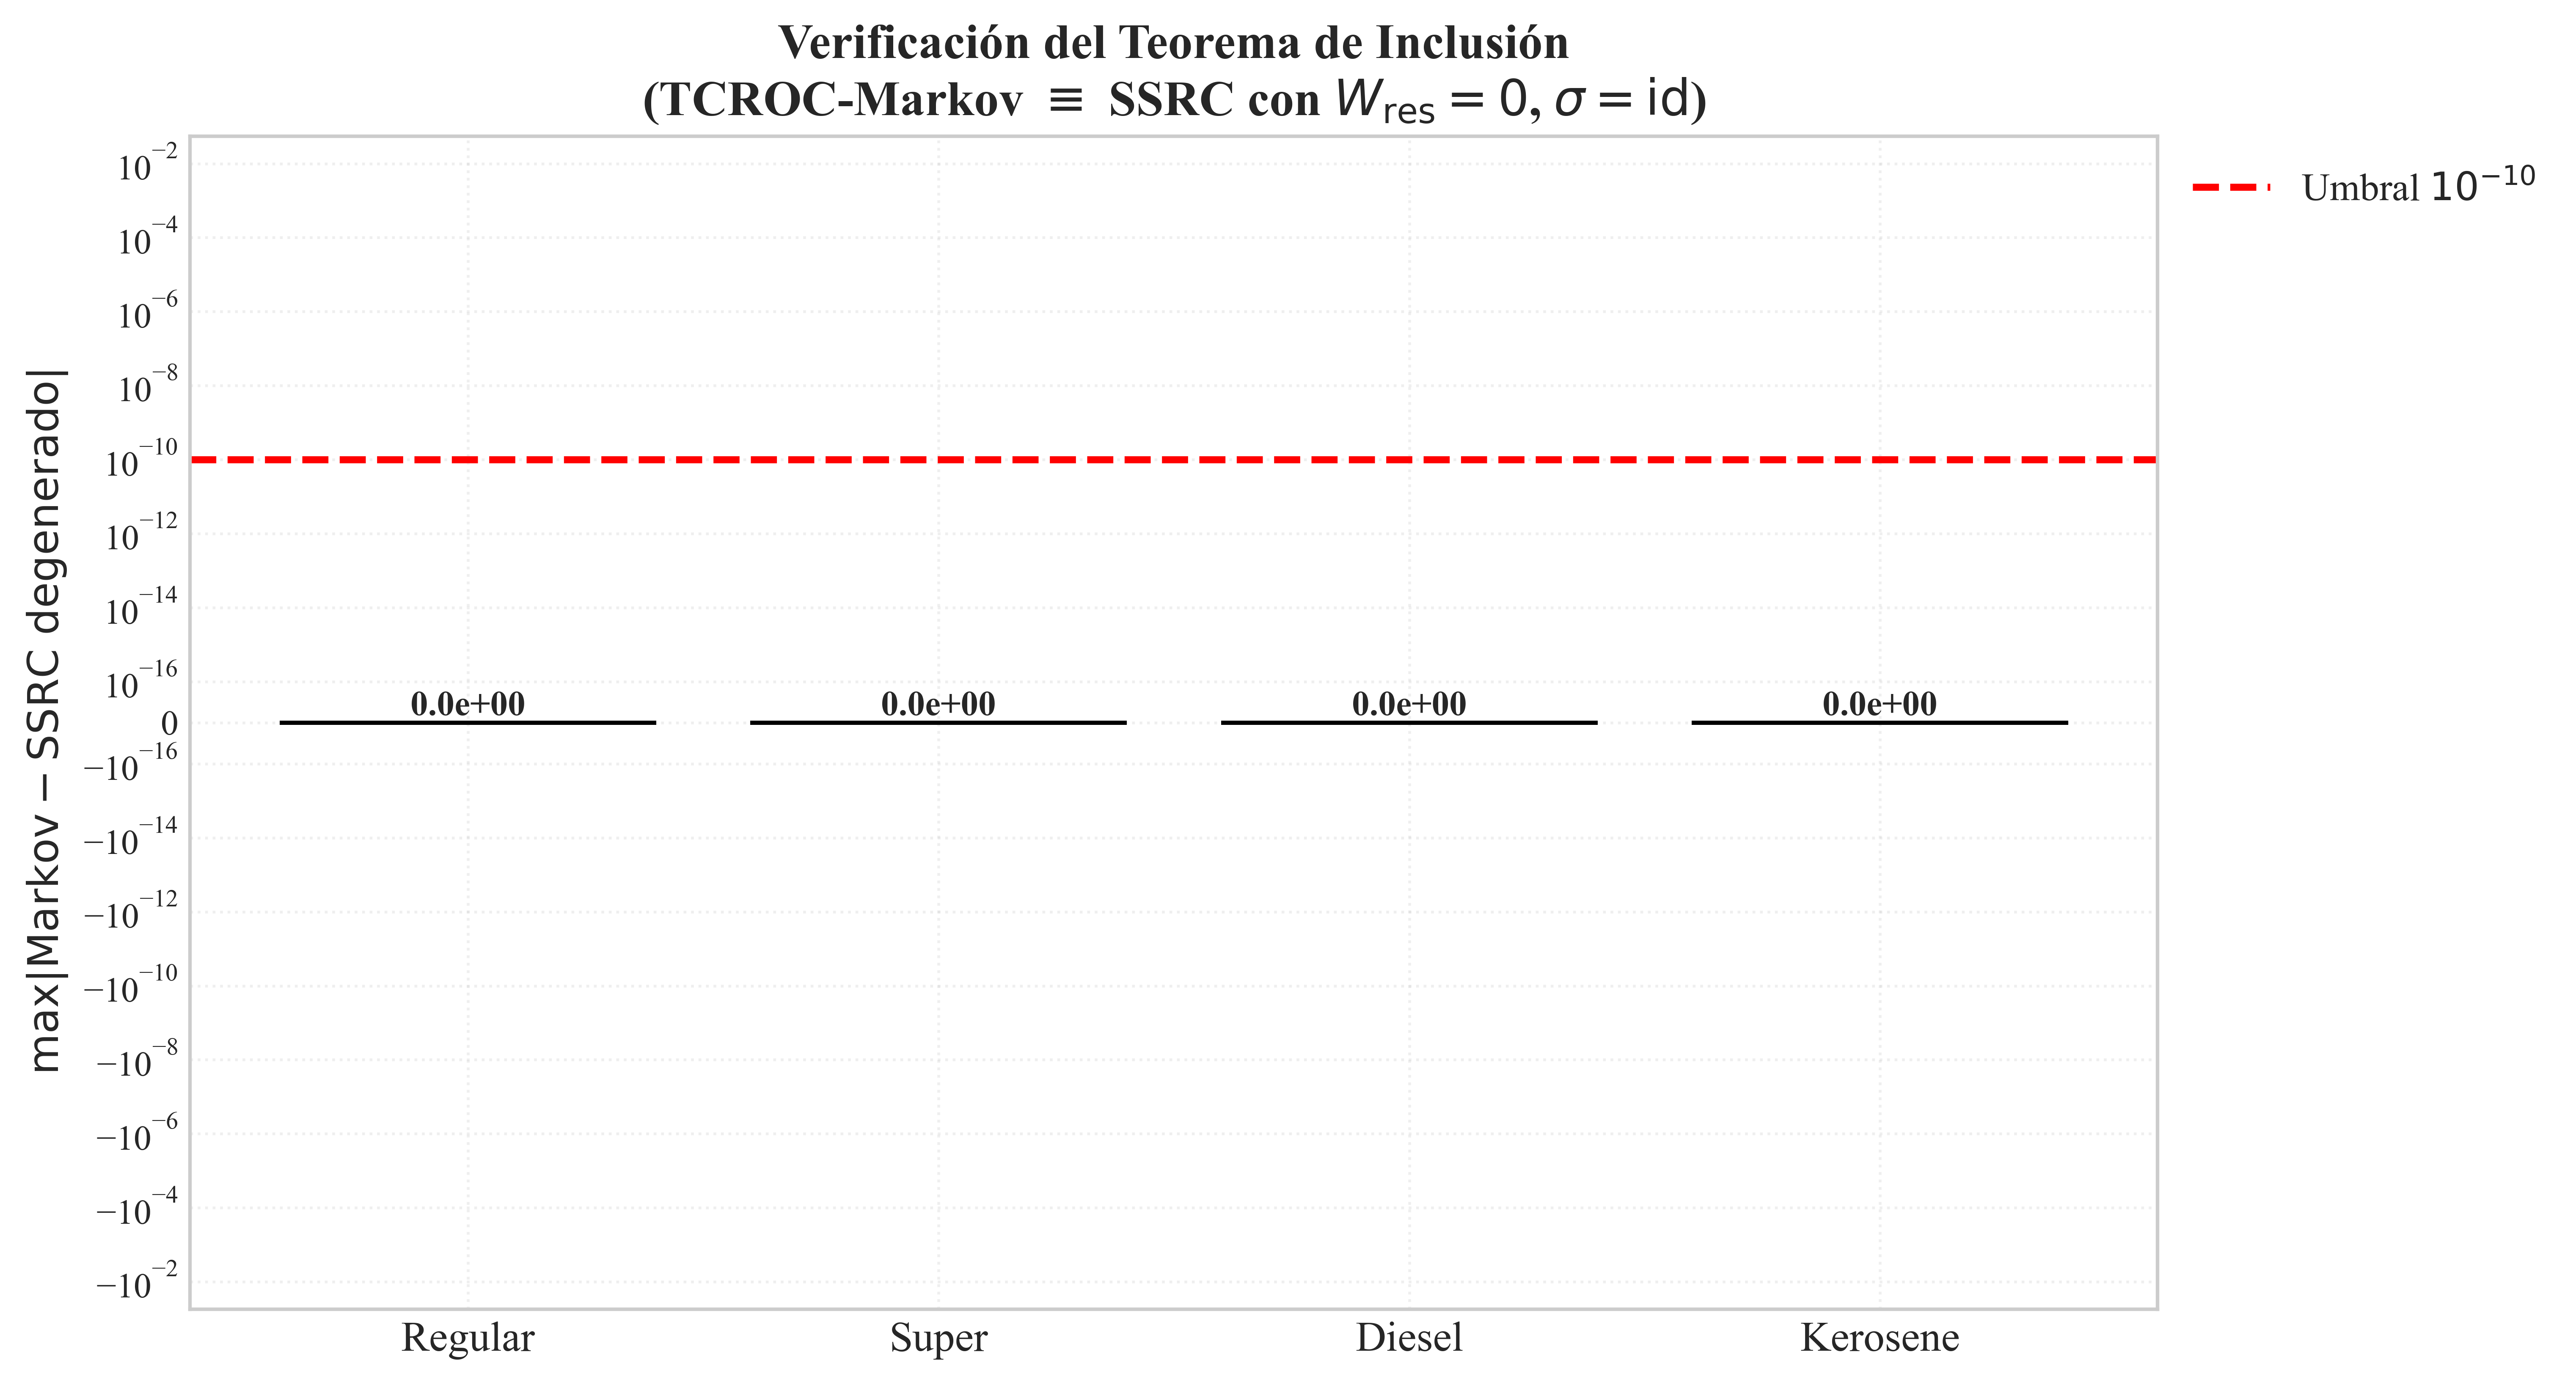
\includegraphics[width=0.95\textwidth]{figures/02_inclusion_theorem.png}
\caption{Verificación de la identidad algebraica entre TCROC-Markov y SSRC degenerado.}
\label{fig:ssrc_inclusion}
\end{figure}

La Figura~\ref{fig:ssrc_inclusion} muestra la verificación numérica del teorema de 
inclusión. Se contrastan las salidas del modelo lineal de Markov con las de 
un reservorio configurado con matriz nula y activación identidad. 
El error residual de exactamente $0.0$ confirma que el marco lineal 
es un subconjunto estricto de la arquitectura SSRC, validando la consistencia 
algebraica de la generalización no lineal propuesta.

\begin{corollary}[Jerarquía de modelos]
\label{cor:jerarquia}
El marco TCROC-Markov del
Capítulo~\ref{cap:regimenes_combustibles} es un caso particular
del SSRC (Definición~\ref{def:ssrc}) obtenido al fijar
$\mat{W}_{\text{res}} = \mat{0}$, $\sigma = \mathrm{id}$,
$a = 1$ y $D = K$.  La extensión a $\mat{W}_{\text{res}} \ne \mat{0}$,
$\sigma = \tanh$, $a < 1$ y $D > K$ constituye una generalización
estrictamente más expresiva: por el
Teorema~\ref{teo:aproximacion_universal}, el SSRC puede aproximar
cualquier funcional causal continuo sobre secuencias, mientras que
TCROC-Markov está restringido a dependencias lineales sobre estados
discretos de un paso.
\end{corollary}

\begin{proof}
La primera afirmación es consecuencia directa del
Teorema~\ref{teo:inclusion}.  Para la segunda, basta observar que
el conjunto de funciones realizables por TCROC-Markov (composiciones
lineales de indicadoras de pertenencia a clústeres) es un subconjunto
propio del conjunto de funcionales continuos sobre
$\set{U}^{\mathbb{Z}_{-}}$.  La densidad del segundo en la
topología del producto está garantizada por el
Teorema~\ref{teo:aproximacion_universal}.
\end{proof}

% --- SECCIÓN: Estimación de la Capa de Lectura vía NNLS ---
\section{Estimación de la Capa de Lectura vía NNLS}
\label{sec:ssrc_estimacion_nnls}
% ===================================================================

La separación entre reservorio fijo y lectura entrenable permite
reducir la estimación de $\mat{W}_{\text{out}}$ a un problema de
mínimos cuadrados, que en nuestro caso resolvemos bajo la restricción de no negatividad para asegurar que se optimiza siempre de forma positiva y no negativa, lo cual es axiomático para que el vector actúe como una suma convexa de propiedades físicas sin cancelar filtros.

% --- SUBSECCIÓN: Formulación del Problema --- - - - - - - - - - - - - - - - - - - - - - - - - - - - - - -
\subsection{Formulación del Problema}
\label{subsec:formulacion_nnls_ssrc}
% -------------------------------------------------------------------

Dada la secuencia de estados del reservorio
$\{\vect{h}_t\}_{t=W}^{T}$ generada por la señal TCROC
$\{\alpha_t\}$, y los valores objetivo
$\{y_t\}_{t=W+1}^{T}$, se busca la matriz de lectura que
minimiza el error de reconstrucción:
\begin{equation}
    \hat{\mat{W}}_{\text{out}} = \argmin_{\mat{W} \ge \mat{0}}
    \sum_{t=W}^{T-1}
    \|y_{t+1} - \mat{W}\,\vect{h}_t\|^2.
    \label{eq:nnls_ssrc}
\end{equation}

Definiendo la matriz de estados acumulados
$\mat{H} = [\vect{h}_W, \vect{h}_{W+1}, \ldots,
\vect{h}_{T-1}] \in \mathbb{R}^{D \times (T-W)}$ y el vector
de objetivos $\vect{y} = [y_{W+1}, \ldots, y_T]^T$, el
problema~\eqref{eq:nnls_ssrc} se reescribe en forma matricial:
\begin{equation}
    \hat{\vect{w}} = \argmin_{\vect{w} \ge \vect{0}}
    \|\vect{y} - \mat{H}^T\vect{w}\|^2,
    \label{eq:nnls_ssrc_matricial}
\end{equation}
donde $\vect{w} = \text{vec}(\mat{W}_{\text{out}}^T)$.

% --- SUBSECCIÓN: Herencia de las Propiedades NNLS --- - - - - - - - - - - - - - - - - - - - - - - - - - - - - - -
\subsection{Herencia de las Propiedades NNLS}
\label{subsec:herencia_nnls}
% -------------------------------------------------------------------

\begin{theorem}[Existencia y unicidad de la capa de lectura NNLS]
\label{teo:existencia_wout}
Sea $\mat{H} \in \mathbb{R}^{D \times (T-W)}$ la matriz de estados
del reservorio.  Entonces:
\begin{enumerate}
    \item \textbf{Existencia:} El
    problema~\eqref{eq:nnls_ssrc_matricial} admite al menos una
    solución.
    \item \textbf{Unicidad:} Si $\mat{H}$ tiene rango completo por
    filas (i.e., $\mathrm{rango}(\mat{H}) = D$), la solución es
    única.
\end{enumerate}
\end{theorem}

\begin{proof}
\textbf{(1) Existencia.}  El conjunto factible
$\set{C} = \{\vect{w} \in \mathbb{R}^{Dm} : \vect{w} \ge \vect{0}\}$
es un cono convexo cerrado no vacío ($\vect{0} \in \set{C}$).  La
función objetivo $f(\vect{w}) = \|\vect{y} - \mat{H}^T\vect{w}\|^2$
es continua y coerciva en $\set{C}$.  Por el teorema de
Weierstrass, $f$ alcanza su mínimo en $\set{C}$.

\textbf{(2) Unicidad.}  Si $\mathrm{rango}(\mat{H}) = D$, entonces
$\mat{H}\mat{H}^T$ es definida positiva, lo que implica que
$f(\vect{w}) = \vect{w}^T(\mat{H}\mat{H}^T)\vect{w} -
2\vect{y}^T\mat{H}^T\vect{w} + \|\vect{y}\|^2$ es estrictamente
convexa en $\vect{w}$.  Un funcional estrictamente convexo sobre un
conjunto convexo tiene a lo sumo un minimizador.  Combinado con la
existencia del punto (1), la solución es única.
\end{proof}

\begin{remark}[Condición de rango y condicionamiento numérico]
\label{obs:condicion_rango}
La condición $\mathrm{rango}(\mat{H}) = D$ requiere $T - W \ge D$ y
que los estados del reservorio sean linealmente independientes.  La no
linealidad de $\tanh$ y la aleatoriedad de
$\mat{W}_{\text{in}}, \mat{W}_{\text{res}}$ garantizan que esta
condición se satisface genéricamente cuando $T - W > D$.  Sin embargo,
la \emph{unicidad teórica} no implica \emph{estabilidad numérica}:
si el número de condición $\kappa(\mat{H}) = \sigma_{\max}/\sigma_{\min}$
es grande, la solución NNLS puede ser sensible a perturbaciones en
los datos.  En la práctica, la restricción de no negatividad del NNLS
actúa como una regularización implícita que mitiga parcialmente este
efecto, y el promediado sobre múltiples realizaciones
(\textit{ensemble}) lo reduce adicionalmente.  El análisis empírico
del condicionamiento se presenta en la
Sección~\ref{subsec:verificaciones_teoricas}.
\end{remark}

% --- SECCIÓN: Arquitectura TCROC-SSRC ---
\section{Arquitectura TCROC-SSRC}
\label{sec:arquitectura_tcroc_ssrc}
% ===================================================================

La Figura~\ref{fig:ssrc_architecture} presenta la comparación
esquemática de ambas arquitecturas, evidenciando que los pasos 1--2
(extracción TCROC) y 4 (estimación NNLS) son compartidos; la
diferencia reside exclusivamente en el paso 3: discretización K-Means
en TCROC-Markov vs.\ proyección al reservorio recurrente en
TCROC-SSRC.

\begin{figure}[H]
\centering
\includegraphics[width=0.95\textwidth]{figures/01_architecture_diagram.png}
\caption{Comparación esquemática de las arquitecturas TCROC-Markov y TCROC-SSRC.}
\label{fig:ssrc_architecture}
\end{figure}

Como se detalla en el diagrama de la Figura~\ref{fig:ssrc_architecture}, 
ambos marcos tecnológicos comparten la fase inicial de extracción de 
características y la fase final de estimación por mínimos cuadrados. 
La distinción radica en el procesamiento de la información en el espacio de estados, 
donde el modelo SSRC sustituye la discretización por clústeres por una proyección
 a un espacio continuo recurrente de alta dimensión, permitiendo capturar 
 dependencias temporales no lineales inaccesibles para el modelo lineal.

\begin{definition}[Marco TCROC-SSRC]
\label{def:marco_tcroc_ssrc}
El \textbf{marco TCROC-SSRC} para pronóstico de series temporales
consiste en el flujo secuencial:
\begin{enumerate}
    \item \textbf{Extracción TCROC:} Dada la serie $\{v_t\}$, se
    computa la señal $\alpha_t = \alpha_t(W, \lambda)$ según la
    ecuación~\eqref{eq:alpha_t_combustibles} del
    Capítulo~\ref{cap:regimenes_combustibles}.
    \item \textbf{Proyección al reservorio:} Se define la entrada
    $u_t = \alpha_t \in \mathbb{R}$ y se propaga mediante la
    ecuación Leaky-ESN~\eqref{eq:leaky_esn}, con $\vect{h}_0 = \vect{0}$
    y los primeros $W_{\text{wash}}$ pasos descartados
    (\textit{washout}) para eliminar transitorios.
    \item \textbf{Estimación de lectura:} Se resuelve el problema
    NNLS~\eqref{eq:nnls_ssrc} para obtener
    $\hat{\mat{W}}_{\text{out}}$.
    \item \textbf{Pronóstico:} El valor predicho es
    $\hat{y}_{t+1} = \hat{\mat{W}}_{\text{out}}\,\vect{h}_t$.
\end{enumerate}
Los hiperparámetros del marco son: $(W, \lambda)$ heredados de TCROC;
$(D, \rho_{\text{res}}, a, W_{\text{wash}})$ propios del reservorio.
\end{definition}

\begin{proposition}[Consistencia con el caso lineal]
\label{prop:consistencia_lineal}
Con los hiperparámetros del reservorio fijados en
$D = K$, $\mat{W}_{\text{res}} = \mat{0}$, $\sigma = \mathrm{id}$,
$a = 1$ y $W_{\text{wash}} = 0$, el marco TCROC-SSRC se reduce
exactamente al marco TCROC-Markov del
Capítulo~\ref{cap:regimenes_combustibles}.
\end{proposition}

\begin{proof}
Consecuencia directa del Teorema~\ref{teo:inclusion}.
\end{proof}

% --- SECCIÓN: Propiedades de Estabilidad del Pronóstico ---
\section{Propiedades de Estabilidad del Pronóstico}
\label{sec:ssrc_estabilidad}
% ===================================================================

\begin{proposition}[Acotación del error de pronóstico]
\label{prop:acotacion_error}
Sea $\hat{y}_{t+1} = \hat{\mat{W}}_{\text{out}}\,\vect{h}_t$ el
pronóstico del SSRC.  Si el reservorio satisface la ESP con
$\rho(\mat{W}_{\text{res}}) = \rho_{\text{res}} < 1$, entonces
para toda perturbación $\delta\vect{u}_t$ en la entrada con
$\|\delta\vect{u}_t\| \le \epsilon$, la perturbación inducida en
la salida satisface:
\begin{equation}
    \|\delta \hat{y}_{t+1}\| \le
    \|\hat{\mat{W}}_{\text{out}}\|\,
    \frac{\|\mat{W}_{\text{in}}\|\,\epsilon}
    {1 - \rho_{\text{res}}}.
    \label{eq:acotacion_perturbacion}
\end{equation}
\end{proposition}

\begin{proof}
Sea $\{\vect{h}_t\}$ la trayectoria nominal y
$\{\vect{h}_t + \delta\vect{h}_t\}$ la trayectoria perturbada.
Por la Lipschitz continuidad de $\tanh$ con constante $L = 1$:
\begin{equation}
    \|\delta\vect{h}_t\| \le
    \|\mat{W}_{\text{in}}\|\,\|\delta\vect{u}_t\| +
    \|\mat{W}_{\text{res}}\|\,\|\delta\vect{h}_{t-1}\|.
\end{equation}
Si la perturbación es sostenida con
$\|\delta\vect{u}_t\| \le \epsilon$ para todo $t$, iterando
la desigualdad y sumando la serie geométrica:
\begin{equation}
    \sup_t \|\delta\vect{h}_t\| \le
    \frac{\|\mat{W}_{\text{in}}\|\,\epsilon}
    {1 - \rho_{\text{res}}}.
\end{equation}
La cota sobre la salida sigue de la linealidad de la lectura:
$\|\delta\hat{y}_{t+1}\| \le \|\hat{\mat{W}}_{\text{out}}\|\,
\|\delta\vect{h}_t\|$.
\end{proof}

\begin{remark}[Conservadurismo de la cota]
\label{obs:cota_conservadora}
La cota~\eqref{eq:acotacion_perturbacion} es una \emph{cota en el
peor caso} que puede ser significativamente conservadora.  En la
práctica, $\|\hat{\mat{W}}_{\text{out}}\|$ depende fuertemente
del condicionamiento de $\mat{H}$: números de condición altos
producen normas $\|\hat{\mat{W}}_{\text{out}}\|$ grandes,
inflando la cota sin que esto se traduzca necesariamente en
inestabilidad observable.  La restricción de no negatividad del NNLS
restringe $\hat{\mat{W}}_{\text{out}}$ al ortante positivo,
proporcionando una forma de regularización implícita que la cota
teórica no captura.  El análisis empírico de la
Sección~\ref{subsec:sensibilidad_hiperparametros} muestra que la
variabilidad real del pronóstico es órdenes de magnitud menor que
la cota teórica.
\end{remark}

% --- SECCIÓN: Aplicación Comparativa: Combustibles Hondureños ---
\section{Aplicación Comparativa: Combustibles Hondureños}
\label{sec:ssrc_aplicacion}

% --- SUBSECCIÓN: Configuración Experimental --- - - - - - - - - - - - - - - - - - - - - - - - - - - - - - -
\subsection{Configuración Experimental}
\label{subsec:ssrc_configuracion}
% -------------------------------------------------------------------

Los hiperparámetros TCROC se fijaron en los valores óptimos
identificados en la Tabla~\ref{tab:hiperparametros_optimos} del
capítulo anterior.  Para el reservorio, se evaluó una búsqueda
exhaustiva en grilla sobre tres hiperparámetros:
\begin{align}
    D &\in \{20, 30, 40, 50, 60, 75, 100, 150\}, \nonumber\\
    \rho_{\text{res}} &\in \{0.70, 0.80, 0.85, 0.90, 0.95, 0.99\}, \quad
    a \in \{0.1, 0.3, 0.5, 0.7, 1.0\},
    \label{eq:grilla_ssrc}
\end{align}
totalizando $8 \times 6 \times 5 = 240$ configuraciones por serie.
Se fijaron $\omega = 1.0$ para la escala de $\mat{W}_{\text{in}}$,
dispersión del 90\% en $\mat{W}_{\text{res}}$, y
$W_{\text{wash}} = 50$ pasos de washout.  Para cada celda de la
grilla, se evaluaron 5 realizaciones independientes de las matrices
aleatorias, seleccionando el mejor $(D^*, \rho^*, a^*)$ por RMSE
medio.  La evaluación final de la configuración óptima se realizó
con un ensemble de 30 realizaciones independientes para obtener
estimaciones robustas de la media y la variabilidad.

% --- SUBSECCIÓN: Verificaciones Teóricas --- - - - - - - - - - - - - - - - - - - - - - - - - - - - - - -
\subsection{Verificaciones Teóricas}
\label{subsec:verificaciones_teoricas}
% -------------------------------------------------------------------

Antes de reportar los resultados predictivos, se verificaron las
condiciones teóricas establecidas en las secciones precedentes.  La
Tabla~\ref{tab:verificaciones_teoricas} resume los resultados para
la configuración óptima de cada serie.

\begin{table}[H]
\centering
\caption{Verificación de las condiciones teóricas del SSRC.}
\label{tab:verificaciones_teoricas}
\begin{tabular}{@{}lcccccc@{}}
\toprule
\textbf{Serie} & $D^*$ & $\rho^*$ 
& \textbf{ESP} & $\mathrm{rango}(\mat{H})$ & $T_{\text{eff}}$
& $\kappa(\mat{H})$ \\
\midrule
Regular  & 150 & 0.85 & Sí & 150 & 340 &
$1.47 \times 10^{9}$ \\
Súper    & 150 & 0.70 & Sí & 150 & 338 &
$5.60 \times 10^{10}$ \\
Diésel   & 150 & 0.80 & Sí & 150 & 340 &
$3.28 \times 10^{9}$ \\
Kerosene &  60 & 0.70 & Sí &  60 & 338 &
$1.14 \times 10^{9}$ \\
\bottomrule
\end{tabular}
\end{table}

Las cuatro configuraciones satisfacen la ESP (todos los
$\rho^* < 1$) y la condición de rango completo
($\mathrm{rango}(\mat{H}) = D^*$ en todos los casos).  La
Figura~\ref{fig:ssrc_eigenvalues} visualiza el espectro de
$\mat{W}_{\text{res}}$, confirmando que todos los autovalores se
encuentran estrictamente dentro del círculo unitario.

\begin{figure}[H]
\centering
\includegraphics[width=0.95\textwidth]{figures/04_eigenvalues_complex_plane.png}
\caption{Autovalores de $\mat{W}_{\text{res}}$ en el plano complejo.}
\label{fig:ssrc_eigenvalues}
\end{figure}

La Figura~\ref{fig:ssrc_eigenvalues} muestra los autovalores de 
$\mat{W}_{\text{res}}$ para la configuración óptima de cada serie. 
El círculo negro punteado representa el círculo unitario ($|z| = 1$), 
mientras que el círculo rojo sólido indica el radio espectral objetivo 
$\rho^*$. Se verifica que todos los autovalores se encuentran estrictamente 
dentro del círculo unitario, cumpliendo con la condición suficiente para la 
ESP detallada en el Teorema~\ref{teo:esp_suficiente}. Los radios espectrales 
óptimos moderados ($\rho^* \in [0.70, 0.85]$) indican que el reservorio no 
requiere de memoria máxima para capturar la dinámica de los combustibles.

Los números de condición $\kappa(\mat{H})$ merecen discusión
explícita. Los valores observados, que se sitúan en el orden de $10^9$ a
$10^{10}$, indican que la matriz $\mat{H}\mat{H}^T$ está
pobremente condicionada en sentido numérico.  Esto es una
consecuencia directa de la dimensión $D = 150$ combinada con la
naturaleza de la señal $\alpha_t$, que tiene variabilidad reducida
($|\alpha_t| < 0.02$ típicamente).  Sin embargo, tres factores
mitigan este condicionamiento en la práctica: (i) la restricción
$\vect{w} \ge \vect{0}$ del NNLS actúa como una regularización
implícita, restringiendo la solución al ortante positivo y
eliminando las direcciones negativas que amplifican el error;
(ii) el ensemble de 30 realizaciones promedia sobre diferentes
matrices $\mat{W}_{\text{in}}$ y $\mat{W}_{\text{res}}$, cada
una con condicionamiento diferente; y (iii) los resultados
predictivos (Sección~\ref{subsec:ssrc_resultados}) muestran
variabilidad baja entre realizaciones, evidenciando estabilidad
práctica a pesar del condicionamiento teórico adverso.

La convergencia del periodo de washout se presenta en la
Figura~\ref{fig:ssrc_washout}.

\begin{figure}[H]
\centering
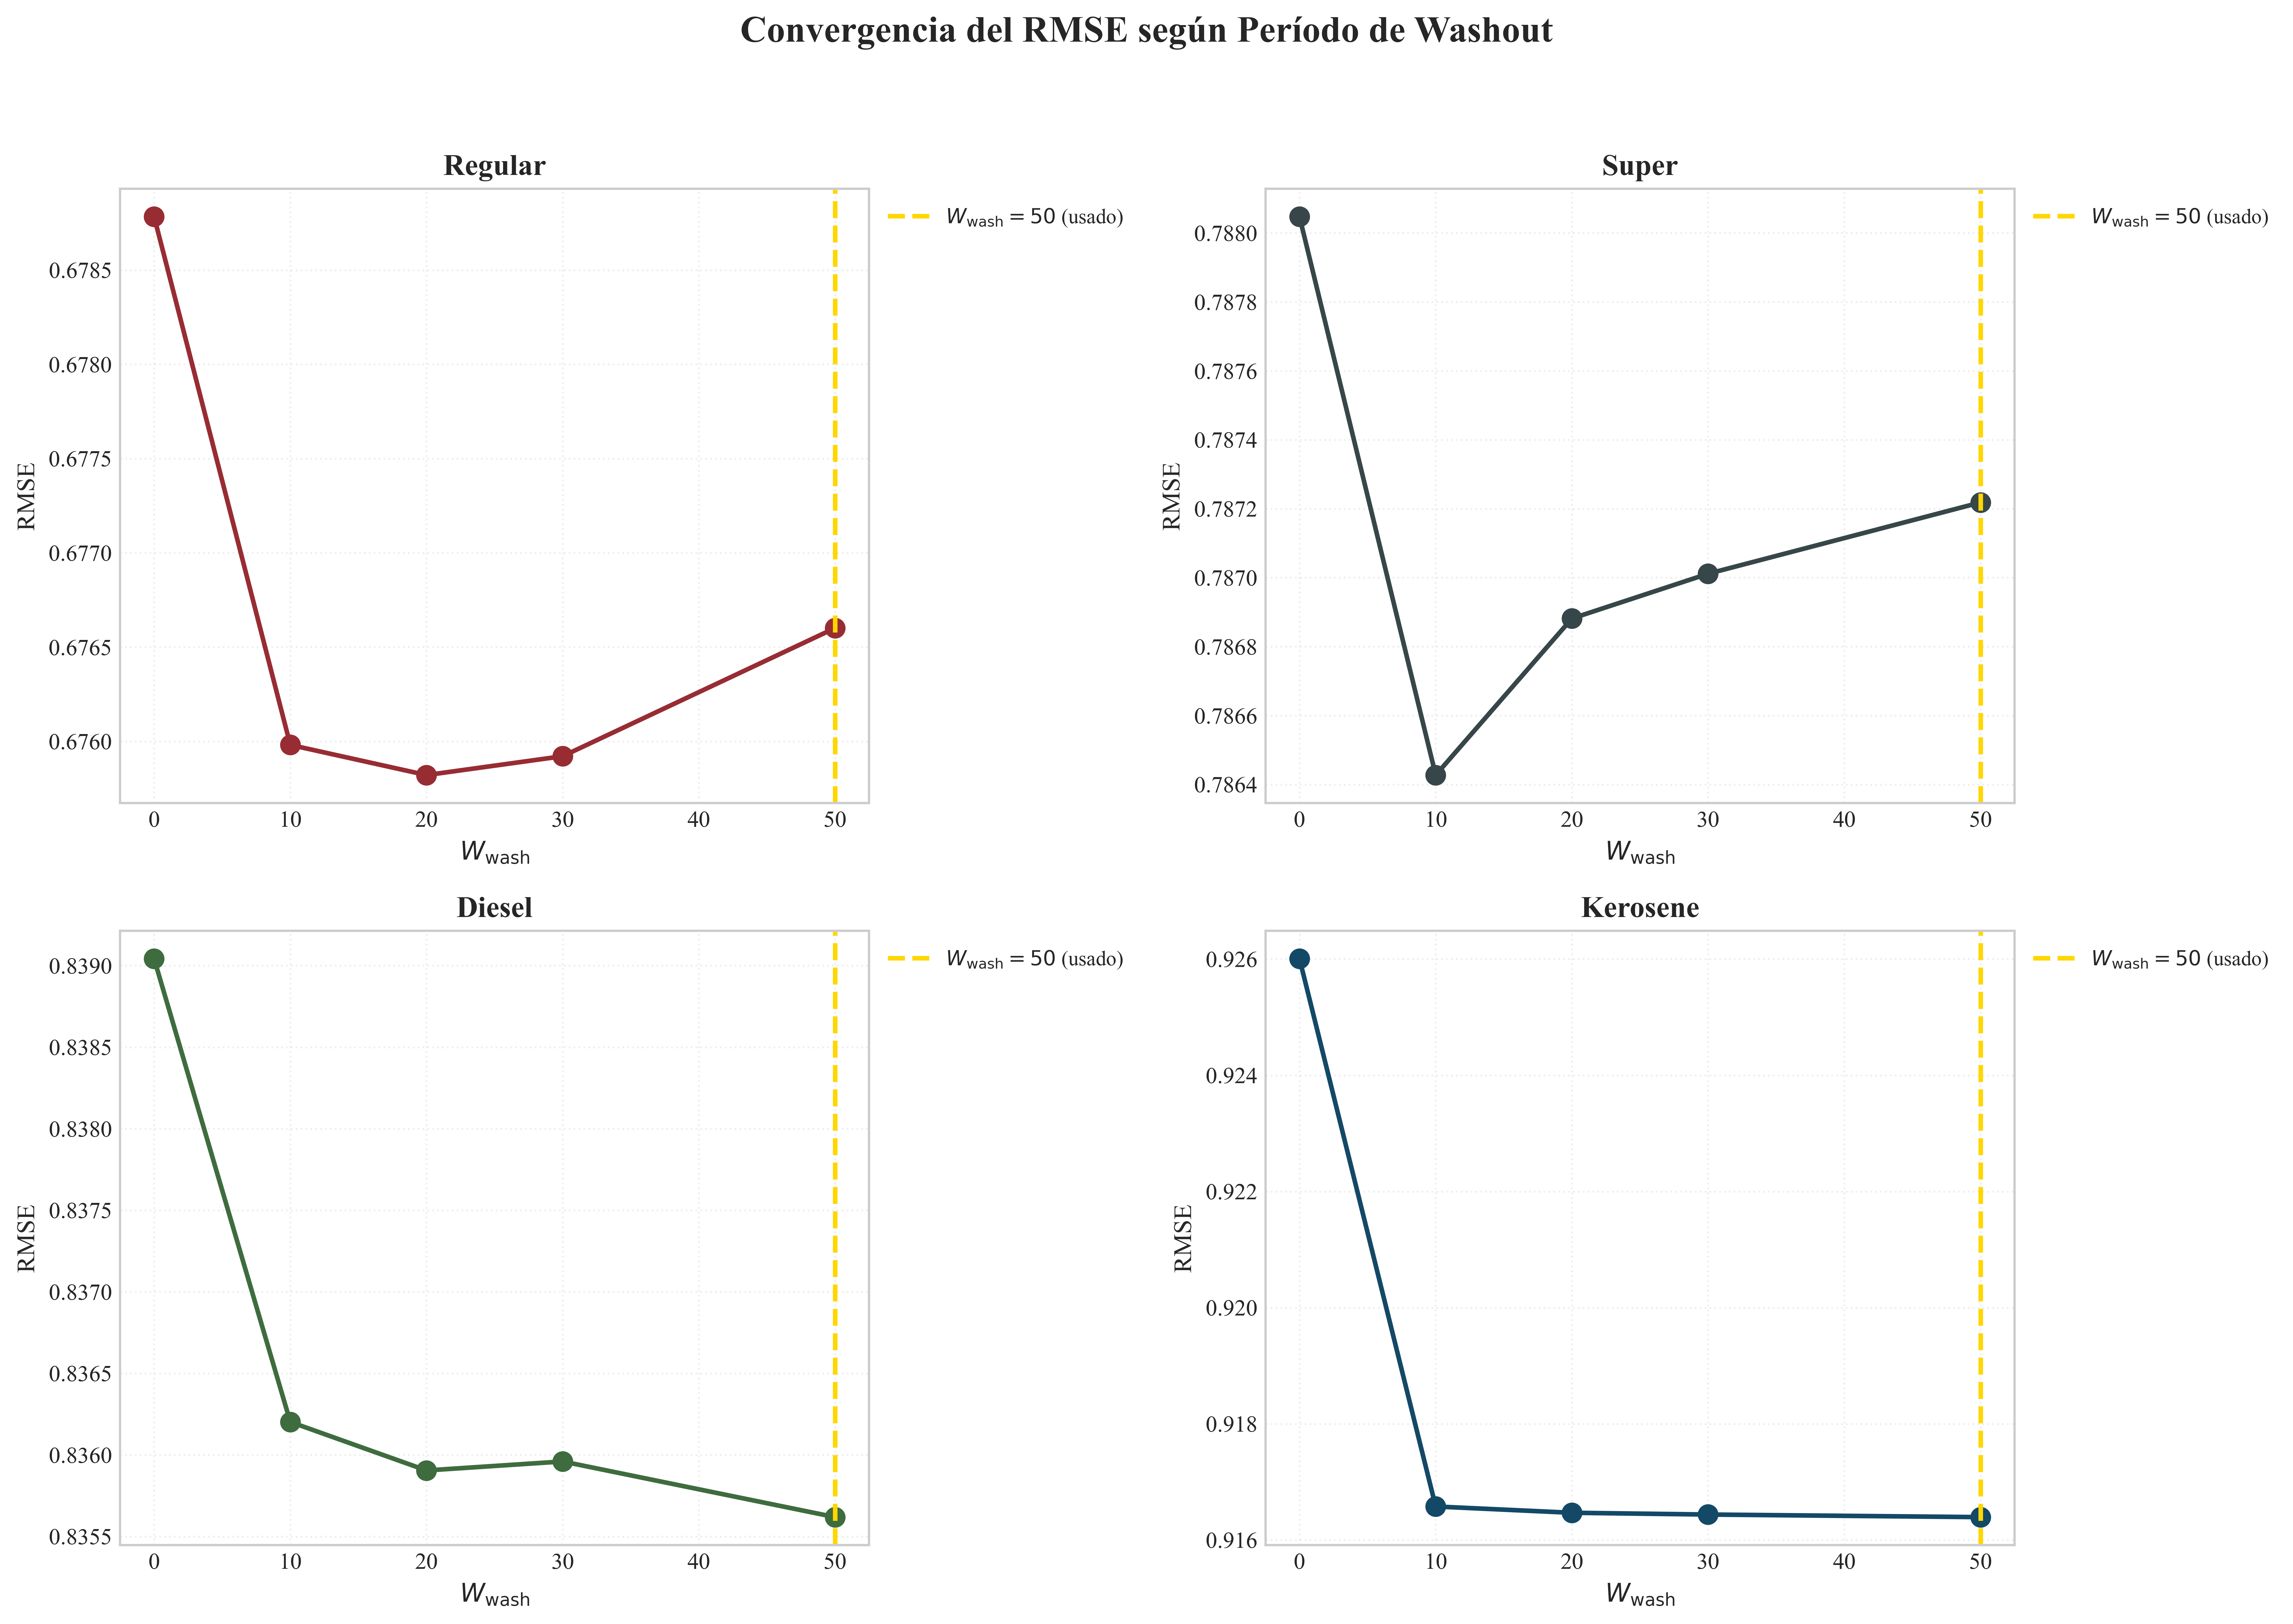
\includegraphics[width=0.95\textwidth]{figures/11_washout_convergence.png}
\caption{Convergencia del RMSE según el periodo de washout $W_{\text{wash}}$.}
\label{fig:ssrc_washout}
\end{figure}

Como se ilustra en la Figura~\ref{fig:ssrc_washout}, el RMSE se estabiliza 
para las cuatro series a partir de un periodo de $W_{\text{wash}} 
\approx 10$--$20$. Esto confirma la eficiencia de la ESP, puesto que la 
influencia de la condición inicial $\vect{h}_0 = \vect{0}$ se disipa rápidamente. 
La línea amarilla punteada señala el valor utilizado de $W_{\text{wash}} = 50$, 
el cual se encuentra dentro de la región de convergencia estable, reflejando el 
decaimiento exponencial rápido asociado a radios espectrales moderados ($\rho^* \le 0.85$).

% --- SUBSECCIÓN: Optimización de Hiperparámetros --- - - - - - - - - - - - - - - - - - - - - - - - - - - - - - -
\subsection{Optimización de Hiperparámetros}
\label{subsec:optimizacion_ssrc}
% -------------------------------------------------------------------

La Figura~\ref{fig:ssrc_heatmap} presenta los resultados de la
búsqueda en grilla como mapas de calor del RMSE medio en el plano
$(D, \rho)$, donde para cada celda se reporta el mejor valor de
$a$ encontrado.

\begin{figure}[H]
\centering
\includegraphics[width=1\textwidth]{figures/03_grid_heatmap.png}
\caption{Búsqueda en grilla del SSRC sobre el plano $(D, \rho)$.}
\label{fig:ssrc_heatmap}
\end{figure}

Los resultados de la búsqueda en grilla presentados en la Figura~\ref{fig:ssrc_heatmap} 
muestran el RMSE medio para cada combinación $(D, \rho)$ y el mejor factor de fuga $a^*$ 
por celda, con el recuadro negro indicando la configuración óptima. Se observa que para Regular,
 Súper y Diésel el óptimo se alcanza en $D = 150$, mientras que para Kerosene ocurre en 
 $D = 60$. Los radios espectrales óptimos son moderados y la superficie de error es suave, 
 manteniendo el RMSE del SSRC significativamente por debajo del modelo Markoviano en todos los paneles.

La Tabla~\ref{tab:hiperparametros_ssrc} resume la configuración
óptima identificada para cada serie.

\begin{table}[H]
\centering
\caption{Hiperparámetros óptimos del SSRC por serie de combustible.}
\label{tab:hiperparametros_ssrc}
\begin{tabular}{@{}lcccccc@{}}
\toprule
\textbf{Serie} & $D^*$ & $\rho^*$ & $a^*$ &
\textbf{NNLS RMSE} & \textbf{Ridge RMSE} &
$\Delta_{\text{solver}}$ \\
\midrule
Regular  & 150 & 0.85 & 0.1 & 0.6595 & 0.6741 & $-2.16\%$ \\
Súper    & 150 & 0.70 & 0.3 & 0.7810 & 0.7885 & $-0.95\%$ \\
Diésel   & 150 & 0.80 & 0.1 & 0.8299 & 0.8443 & $-1.70\%$ \\
Kerosene &  60 & 0.70 & 1.0 & 0.9156 & 0.9173 & $-0.17\%$ \\
\bottomrule
\end{tabular}
\end{table}

Tres observaciones emergen de la optimización.  Primero, los valores
$a^* = 0.1$ para Regular y Diésel indican que el reservorio se
beneficia de una inercia temporal fuerte: el 90\% del estado previo
se preserva en cada paso, actuando como un filtro de suavizado
adaptativo que es consistente con la baja volatilidad semanal de
estos mercados regulados.  Segundo, Kerosene es la única serie con
$a^* = 1.0$ (ESN estándar sin suavizado), coherente con su mayor
volatilidad y complejidad de 5 regímenes identificados en el
capítulo anterior.  Tercero, NNLS supera a Ridge Regression en las
cuatro series, validando empíricamente que la restricción de no
negatividad, la cual garantiza que el pronóstico sea una combinación
positiva de los filtros no lineales del reservorio, aporta
regularización útil.

Las Figuras~\ref{fig:ssrc_sens_D} y~\ref{fig:ssrc_sens_rho}
presentan el análisis de sensibilidad marginal a los hiperparámetros
$D$ y $\rho$, respectivamente.

\begin{figure}[H]
\centering
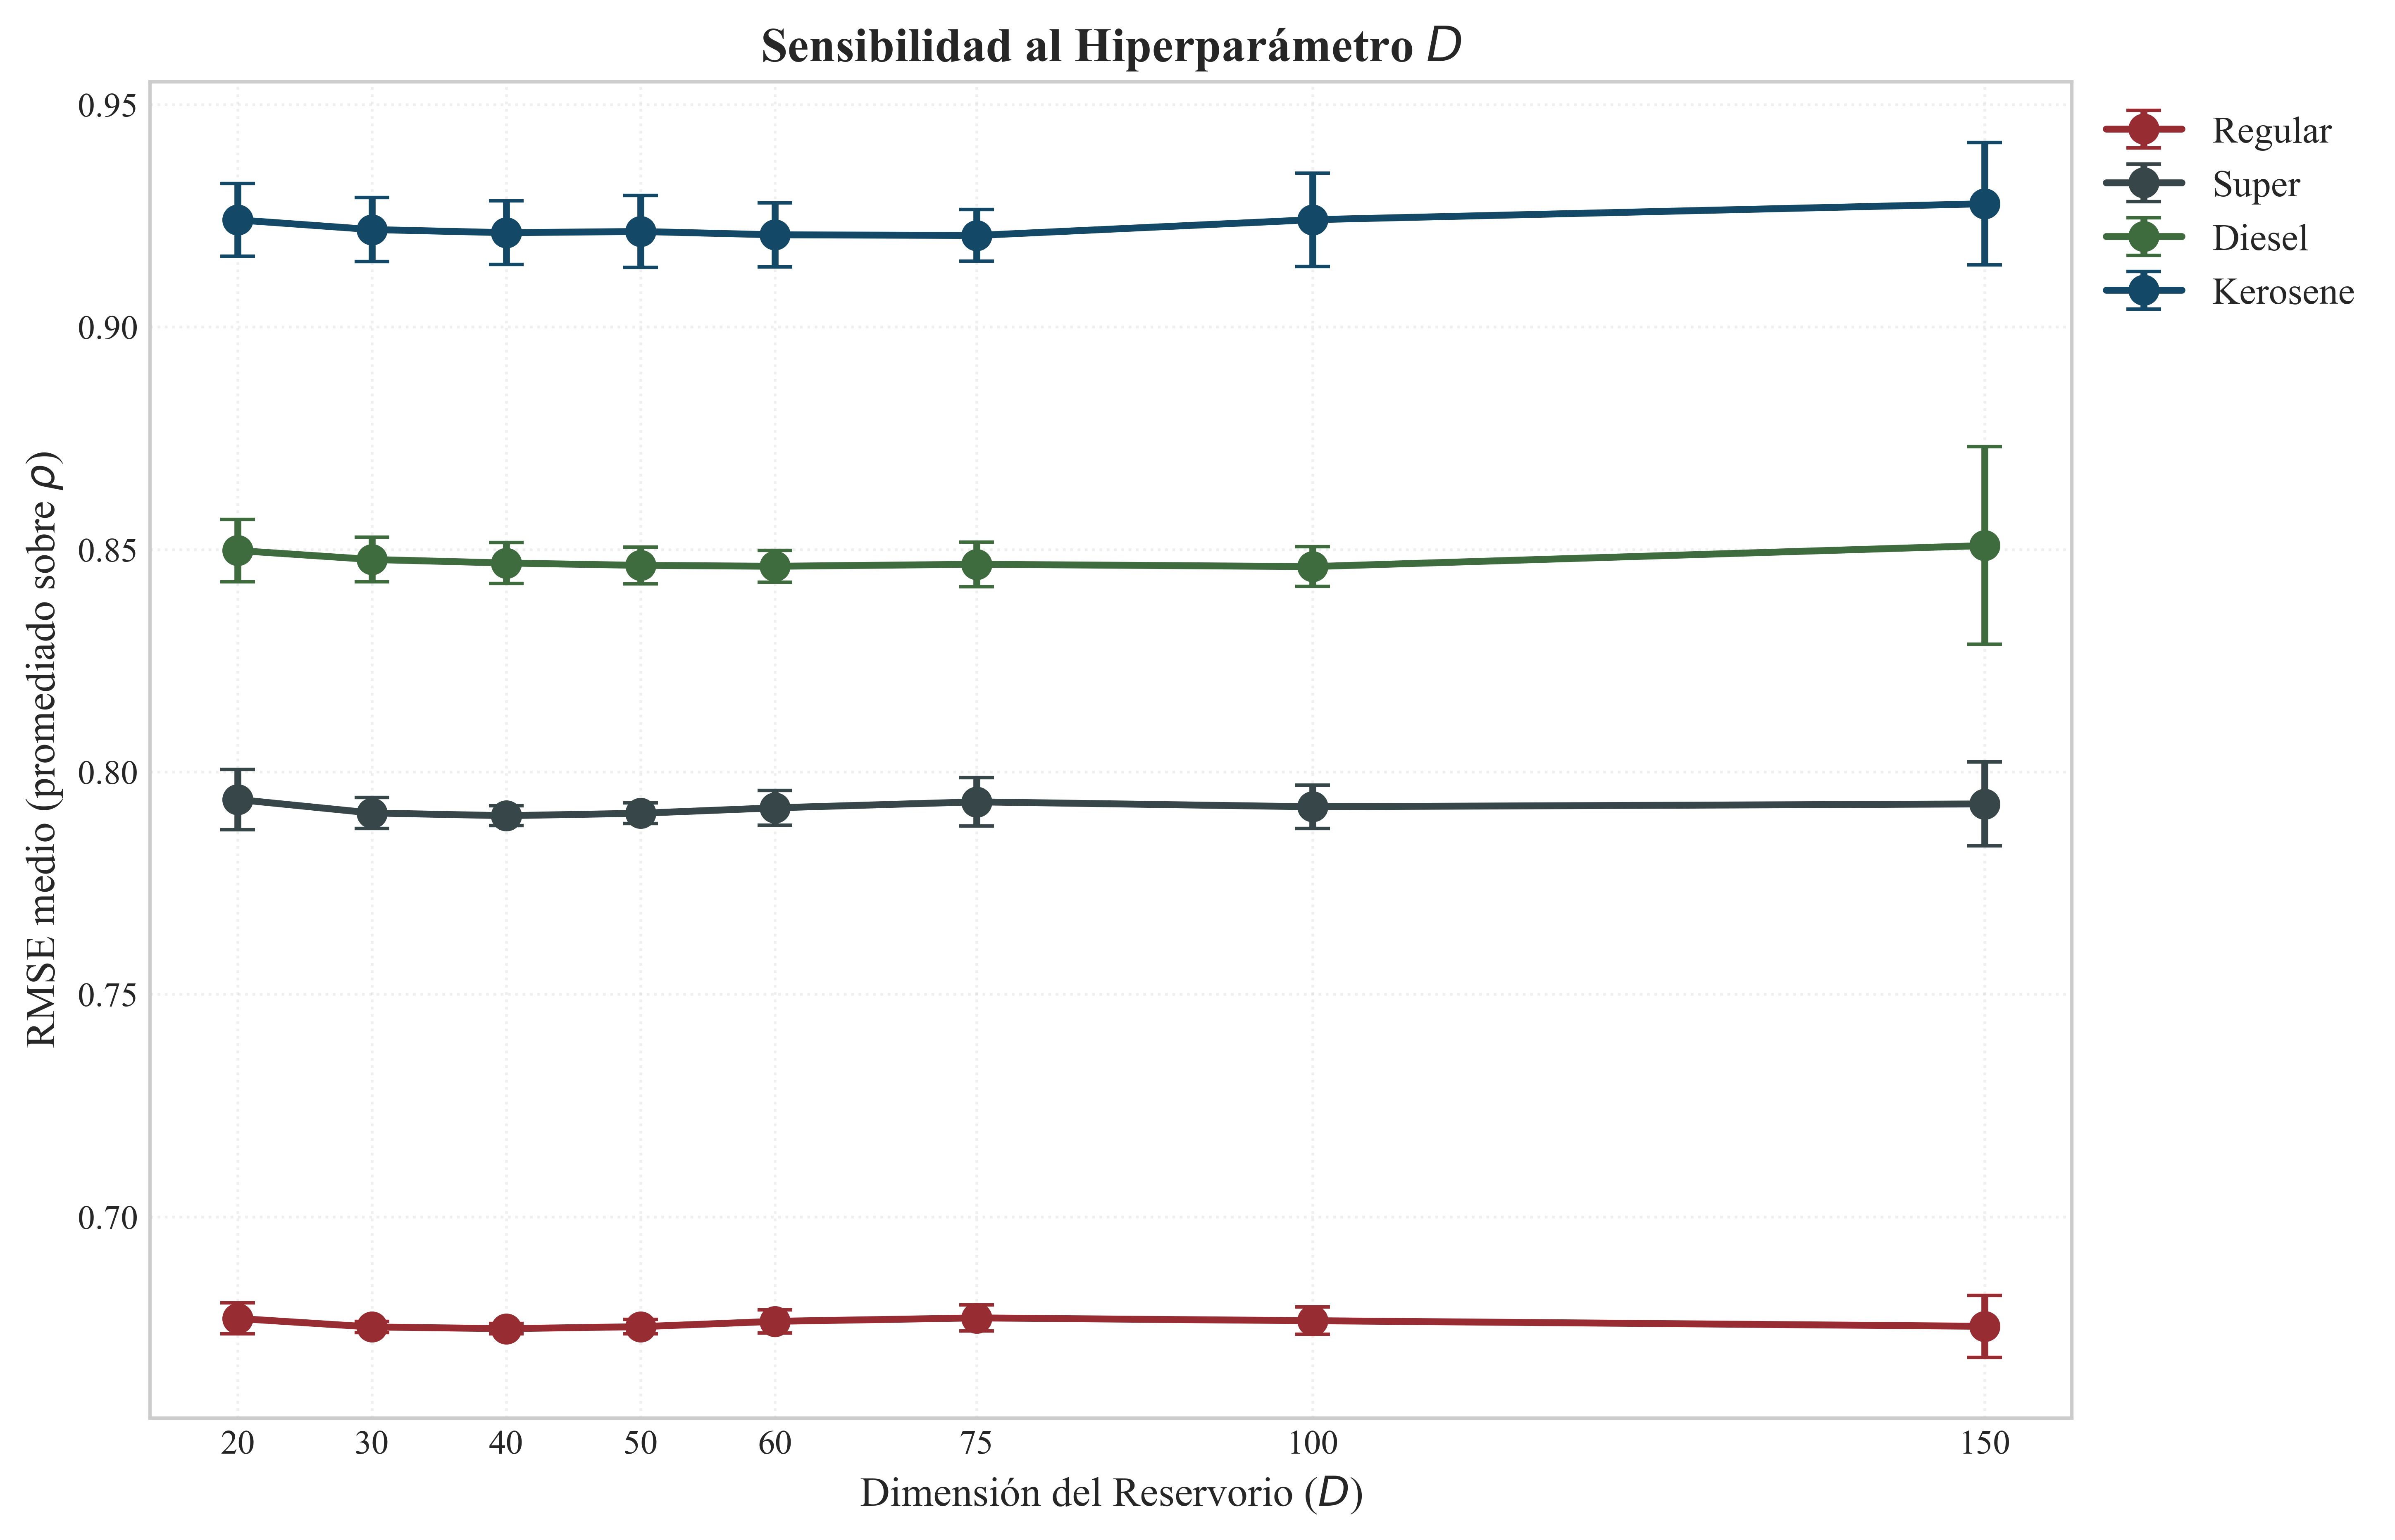
\includegraphics[width=0.95\textwidth]{figures/08_sensitivity_D.png}
\caption{Sensibilidad del RMSE a la dimensión del reservorio $D$.}
\label{fig:ssrc_sens_D}
\end{figure}

La sensibilidad del RMSE respecto a la dimensión $D$ se detalla en la 
Figura~\ref{fig:ssrc_sens_D}. Las curvas promediadas sobre los valores 
de $\rho$ resultan esencialmente planas, con variaciones mínimas entre 
$D = 20$ y $D = 150$. Este comportamiento indica que la complejidad 
no lineal del proceso es baja, permitiendo que incluso dimensiones 
modestas capturen la mayor parte de la estructura, con ganancias 
marginales de apenas el 0.3\% al aumentar la dimensión a los niveles 
máximos evaluados.

\begin{figure}[H]
\centering
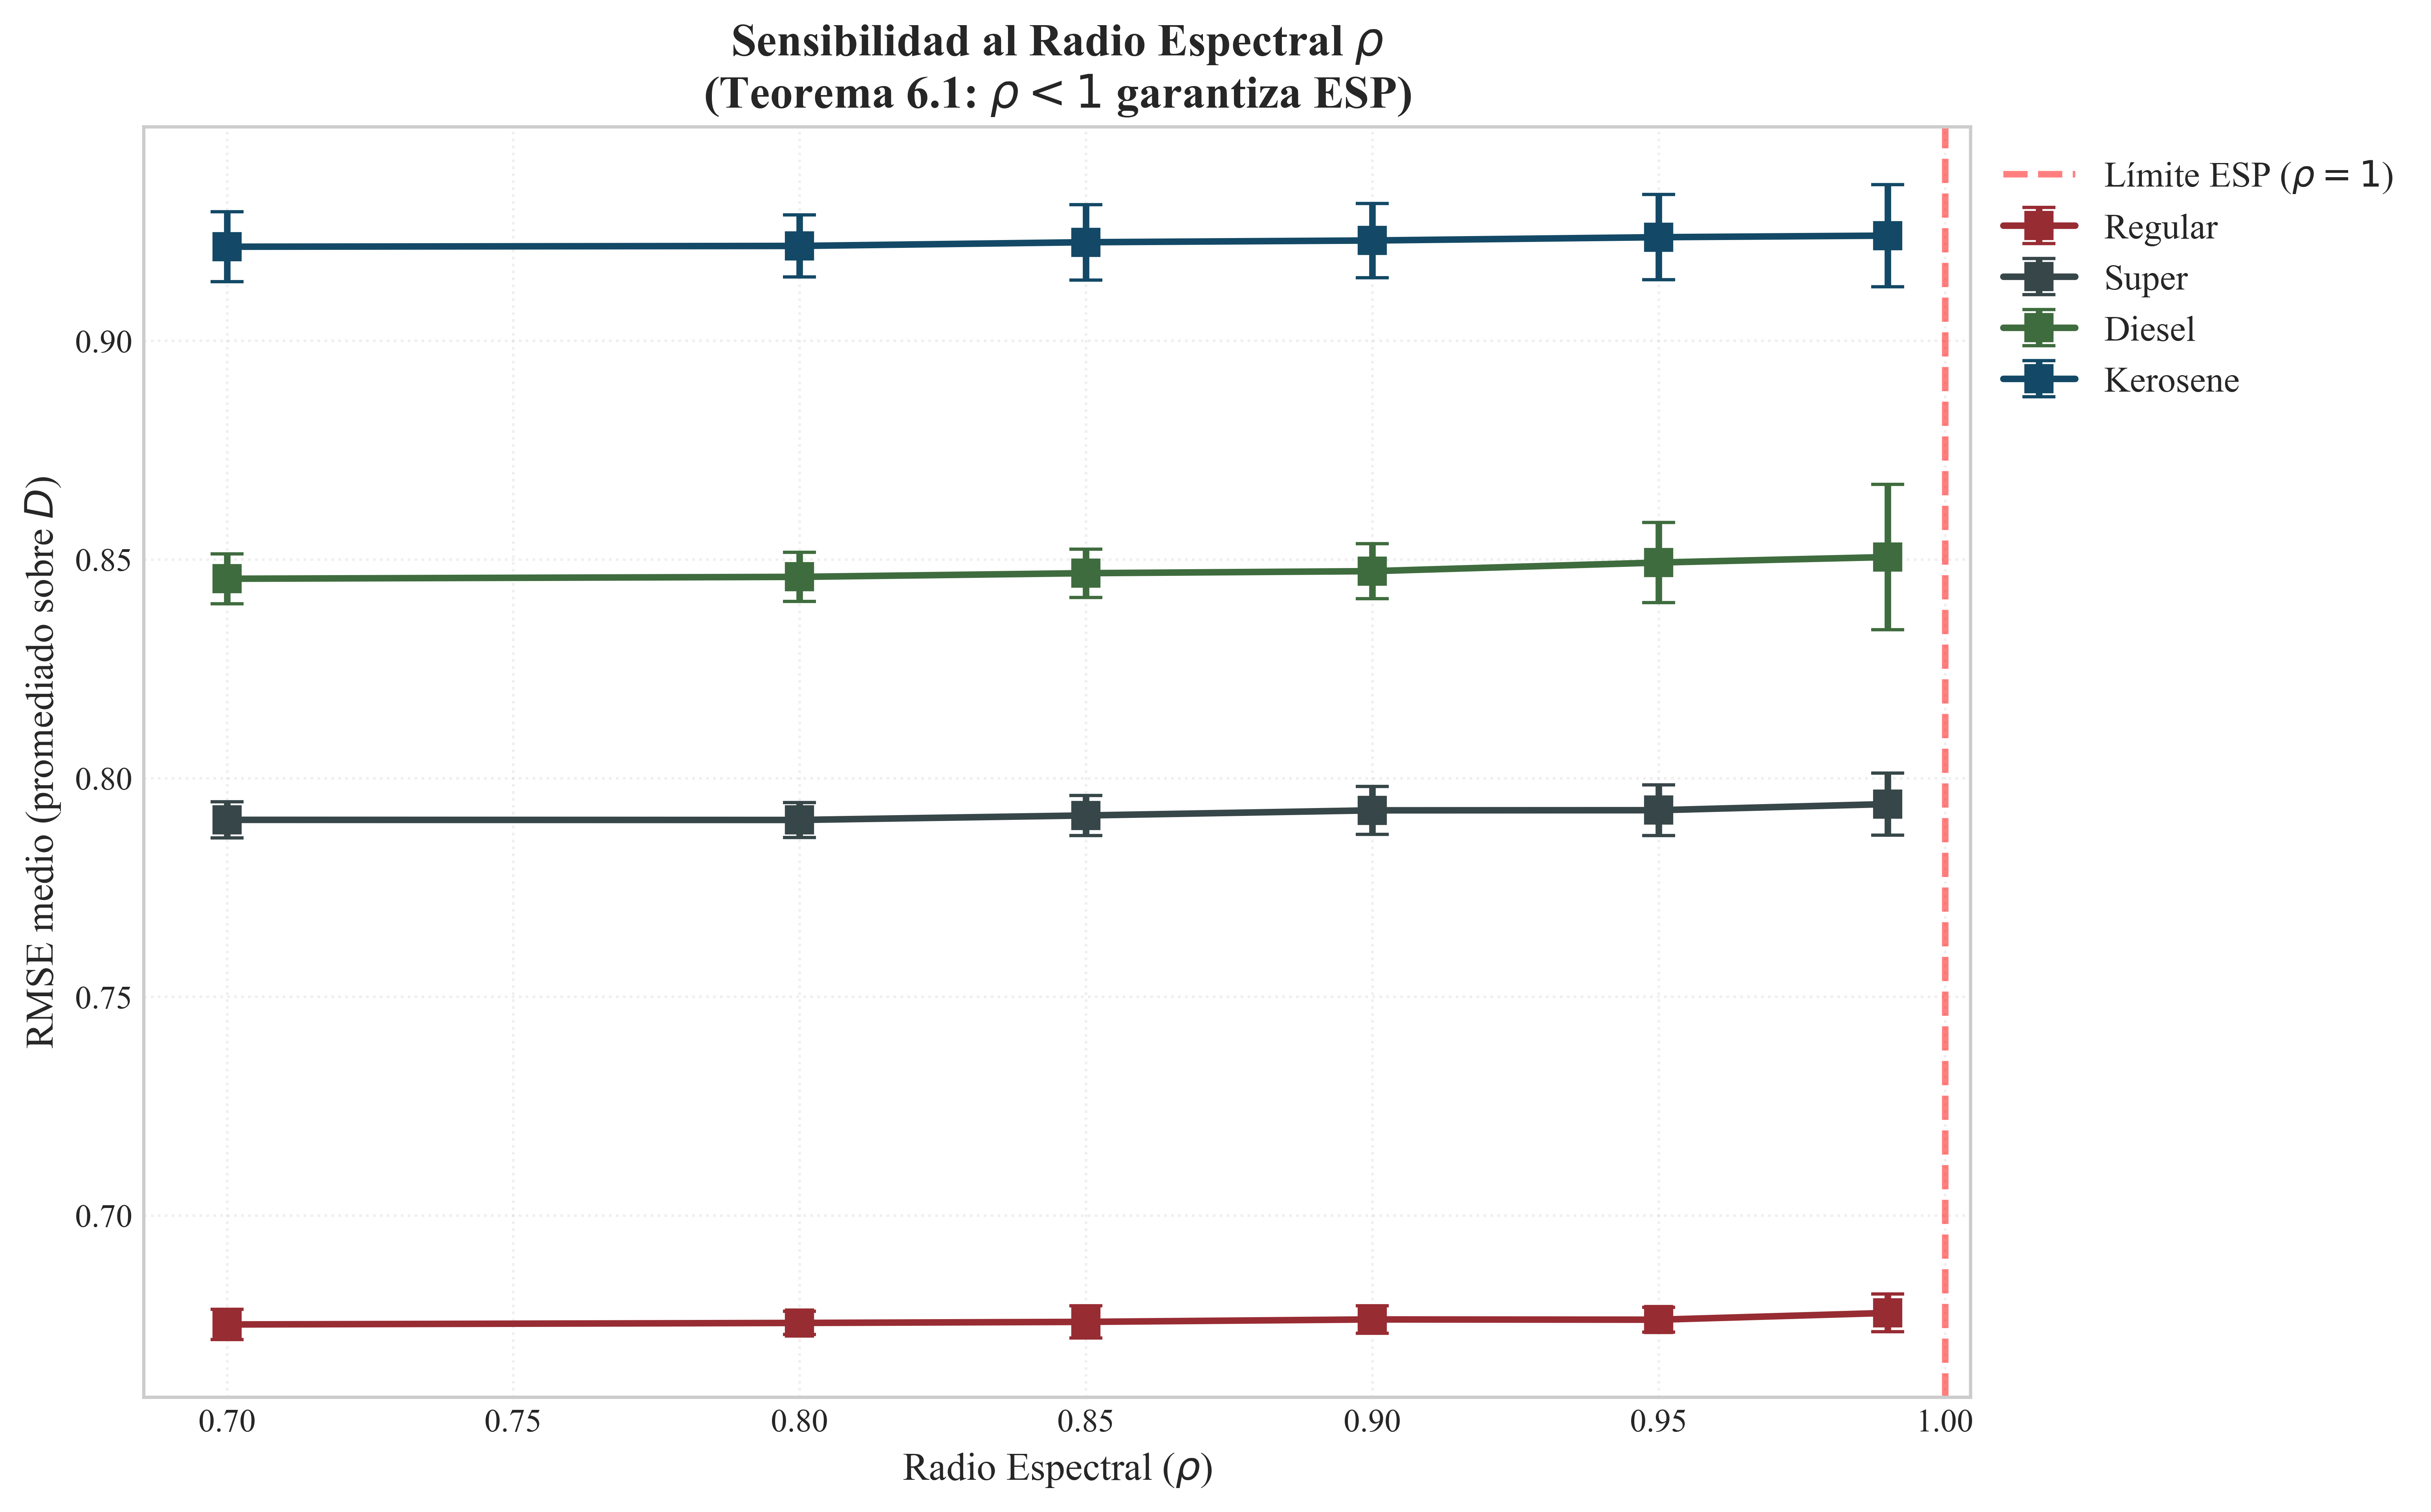
\includegraphics[width=0.95\textwidth]{figures/09_sensitivity_rho.png}
\caption{Sensibilidad del RMSE al radio espectral $\rho$.}
\label{fig:ssrc_sens_rho}
\end{figure}

La Figura~\ref{fig:ssrc_sens_rho} muestra la sensibilidad del RMSE frente 
al radio espectral $\rho$. La tendencia ligeramente creciente hacia 
$\rho = 0.99$ sugiere que un exceso de memoria no lineal no beneficia a 
estas series. Los valores óptimos moderados identificados son consistentes 
con una dinámica dominada por tendencias de largo plazo que ya han sido 
capturadas eficazmente por el operador TCROC.

% --- SUBSECCIÓN: Resultados --- - - - - - - - - - - - - - - - - - - - - - - - - - - - - - -
\subsection{Resultados}
\label{subsec:ssrc_resultados}
% -------------------------------------------------------------------

La Tabla~\ref{tab:comparacion_ssrc} presenta la comparación directa
entre TCROC-Markov y TCROC-SSRC.  La significancia estadística se
evaluó mediante el test de Diebold-Mariano (DM) \cite{dieboldmariano1995},
que compara las secuencias de errores cuadráticos de ambos modelos
bajo la hipótesis nula de igual precisión predictiva.

\begin{table}[H]
\centering
\caption{Comparación de desempeño predictivo: TCROC-Markov vs.\ TCROC-SSRC.}
\label{tab:comparacion_ssrc}
\resizebox{\textwidth}{!}{%
\begin{tabular}{@{}lcccccc@{}}
\toprule
\textbf{Serie} & \textbf{TCROC-Markov} &
\textbf{TCROC-SSRC} & $(D^*, \rho^*, a^*)$ &
$\Delta$\textbf{RMSE} & $p_{\text{DM}}$ &
\textbf{Significativo} \\
\midrule
Regular  & $0.8394$ & $0.6595 \pm 0.013$ &
$(150,\; 0.85,\; 0.1)$ & $-21.43\%$ & $0.1154$ & No \\
Súper    & $0.9769$ & $0.7810 \pm 0.006$ &
$(150,\; 0.70,\; 0.3)$ & $-20.05\%$ & $0.0018$ & Sí \\
Diésel   & $1.0816$ & $0.8299 \pm 0.018$ &
$(150,\; 0.80,\; 0.1)$ & $-23.27\%$ & $0.0326$ & Sí \\
Kerosene & $1.1714$ & $0.9156 \pm 0.005$ &
$(60,\;\, 0.70,\; 1.0)$ & $-21.84\%$ & $0.0061$ & Sí \\
\bottomrule
\end{tabular}%
}
\end{table}

La Tabla~\ref{tab:comparacion_ssrc} presenta la comparación de desempeño predictivo entre TCROC-Markov (lineal) y TCROC-SSRC (no lineal). Se reporta el RMSE fuera de muestra como la media y desviación estándar sobre 30 realizaciones para la extensión SSRC. La significancia estadística, evaluada mediante el test de Diebold-Mariano (DM), muestra que un valor de $p < 0.05$ indica una superioridad significativa del modelo SSRC sobre el benchmark lineal.

El TCROC-SSRC reduce el RMSE entre un 20\% y un 23\% respecto
al modelo Markoviano en las cuatro series.  La mejora es
estadísticamente significativa al nivel $\alpha = 0.05$ para Súper
($p = 0.002$), Diésel ($p = 0.033$) y Kerosene ($p = 0.006$).
Para Regular, la mejora es sustancial en magnitud ($-21.43\%$) pero
marginalmente significativa ($p = 0.115$); esto se atribuye a la
menor varianza de los errores de Regular (la serie más predecible),
que reduce la potencia del test DM.

La Figura~\ref{fig:ssrc_barplot} visualiza esta comparación.

\begin{figure}[H]
\centering
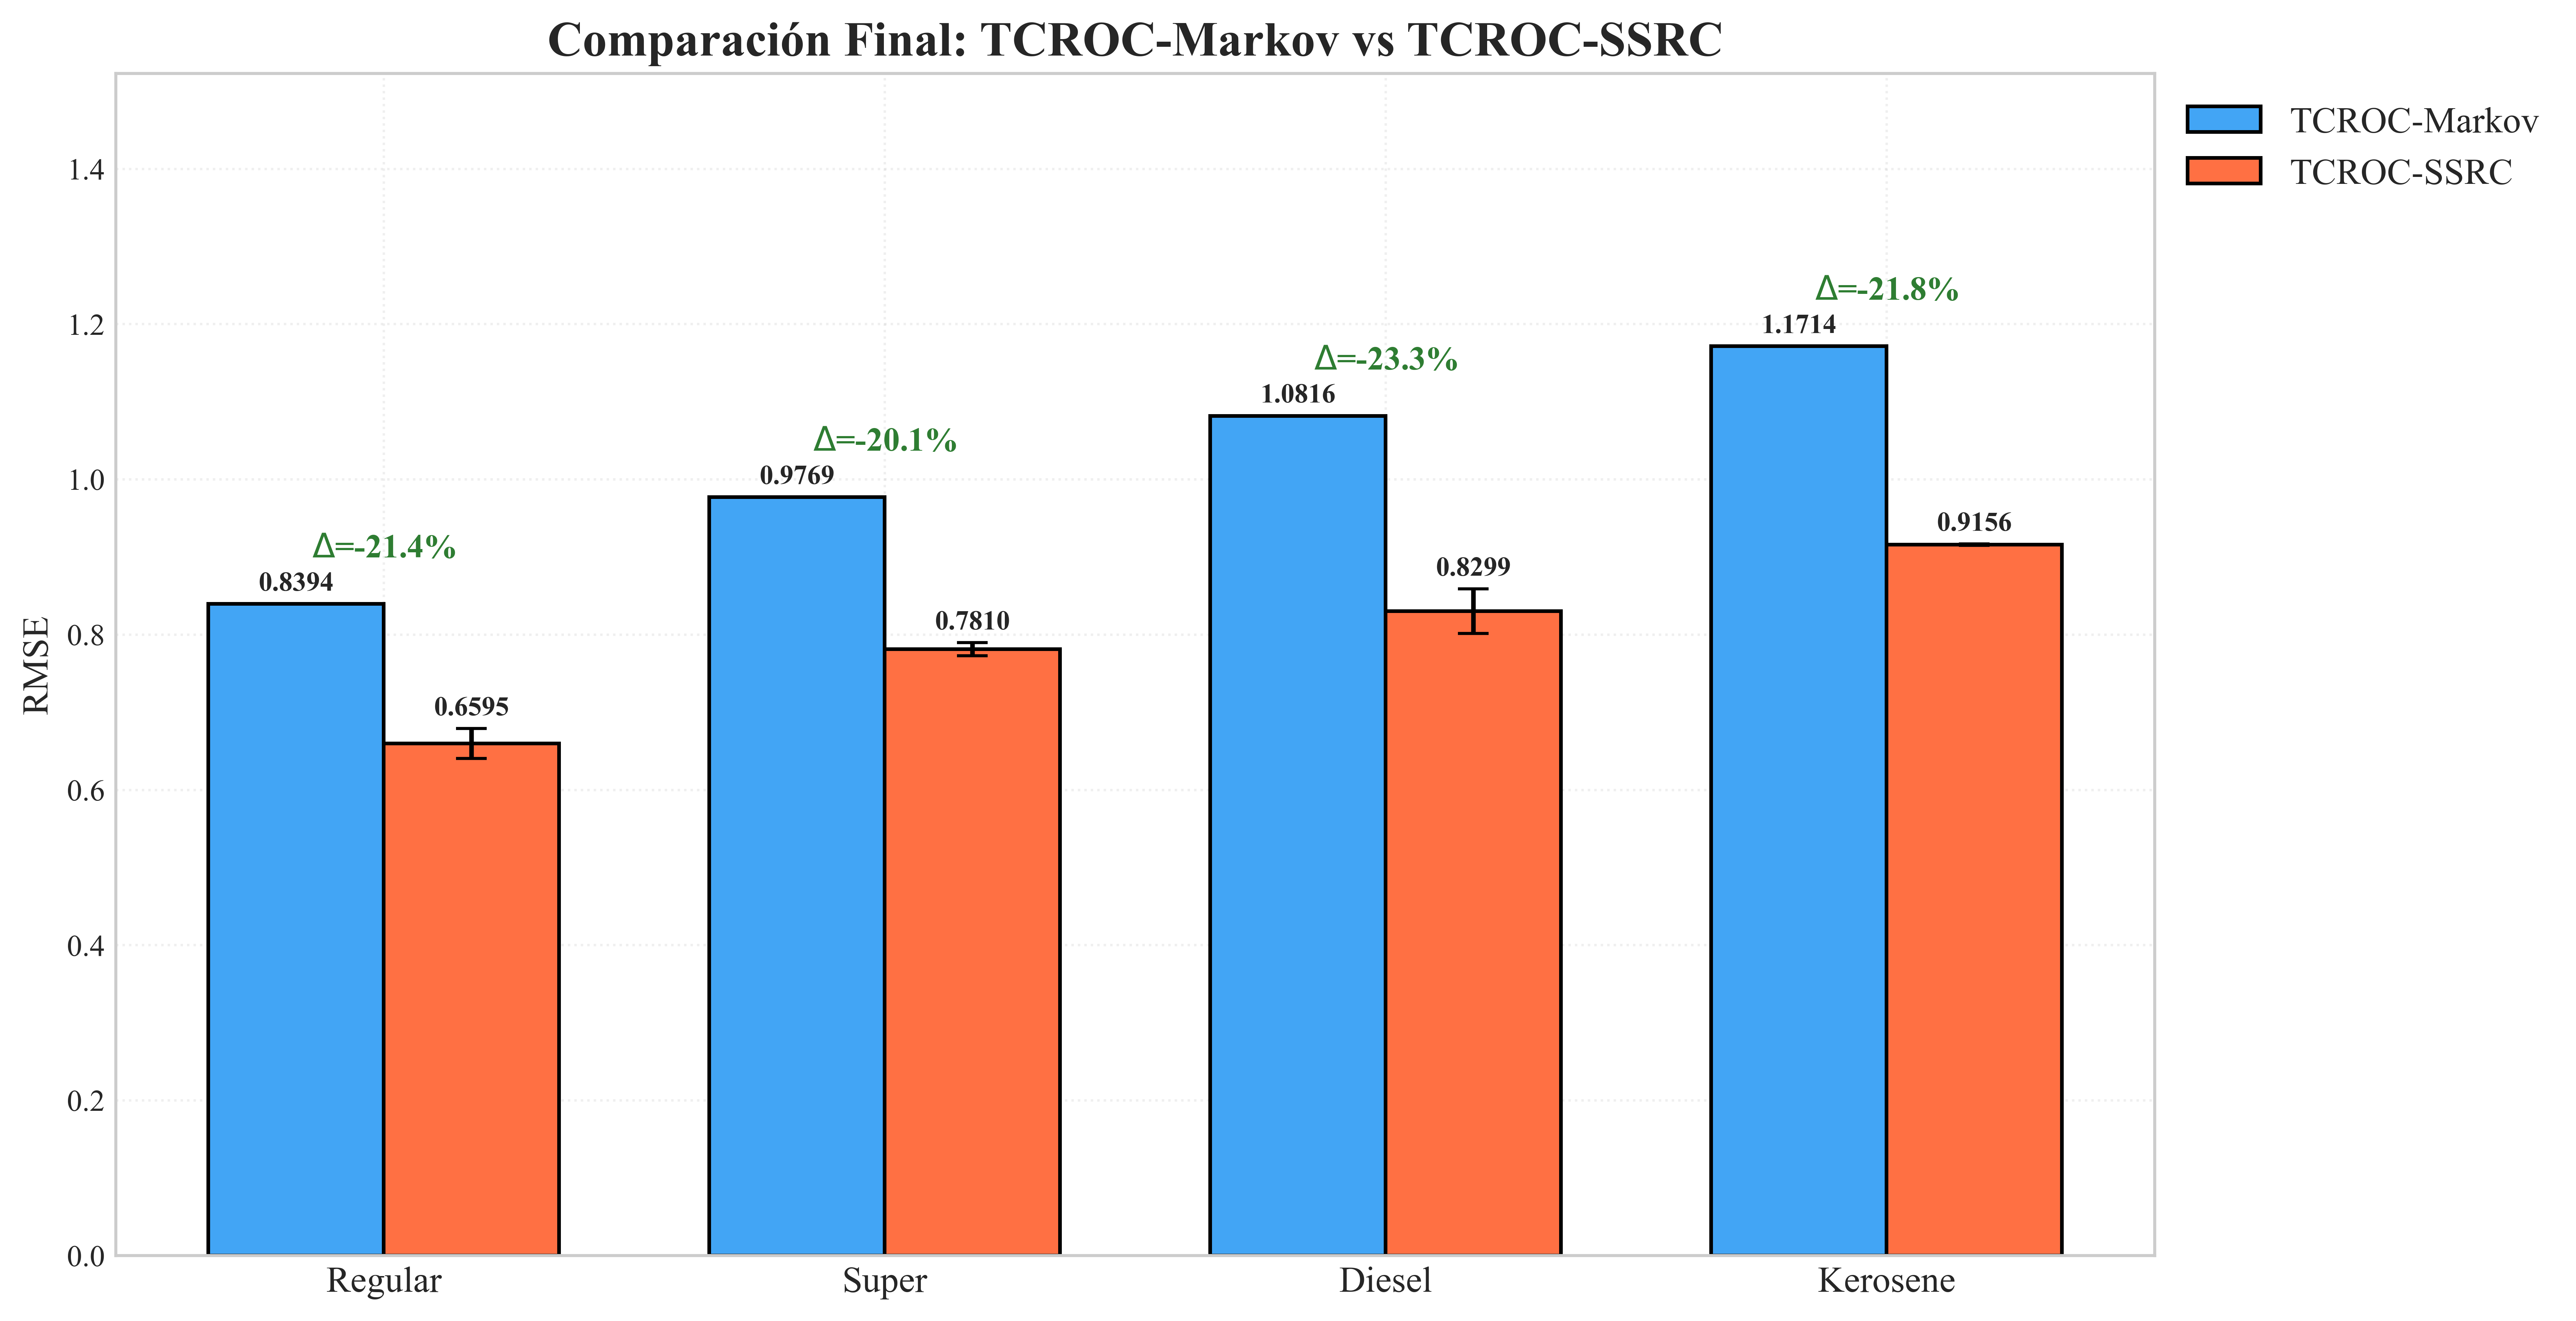
\includegraphics[width=0.95\textwidth]{figures/12_comparison_barplot.png}
\caption{Comparación de RMSE: TCROC-Markov vs.\ TCROC-SSRC.}
\label{fig:ssrc_barplot}
\end{figure}

La Figura~\ref{fig:ssrc_barplot} ofrece una visualización comparativa entre 
TCROC-Markov (azul) y TCROC-SSRC (naranja). Las barras de error para el 
modelo SSRC representan la desviación estándar calculada sobre 30 
realizaciones independientes. La anotación verde resalta la mejora 
porcentual del SSRC, cuya consistencia de entre un 20\% y un 23\% en 
las cuatro series analizadas sugiere un beneficio estructural derivado 
de la extensión no lineal.

La Figura~\ref{fig:ssrc_boxplot} presenta la distribución del RMSE
sobre las 30 realizaciones para cuantificar la variabilidad
estocástica del SSRC.

\begin{figure}[H]
\centering
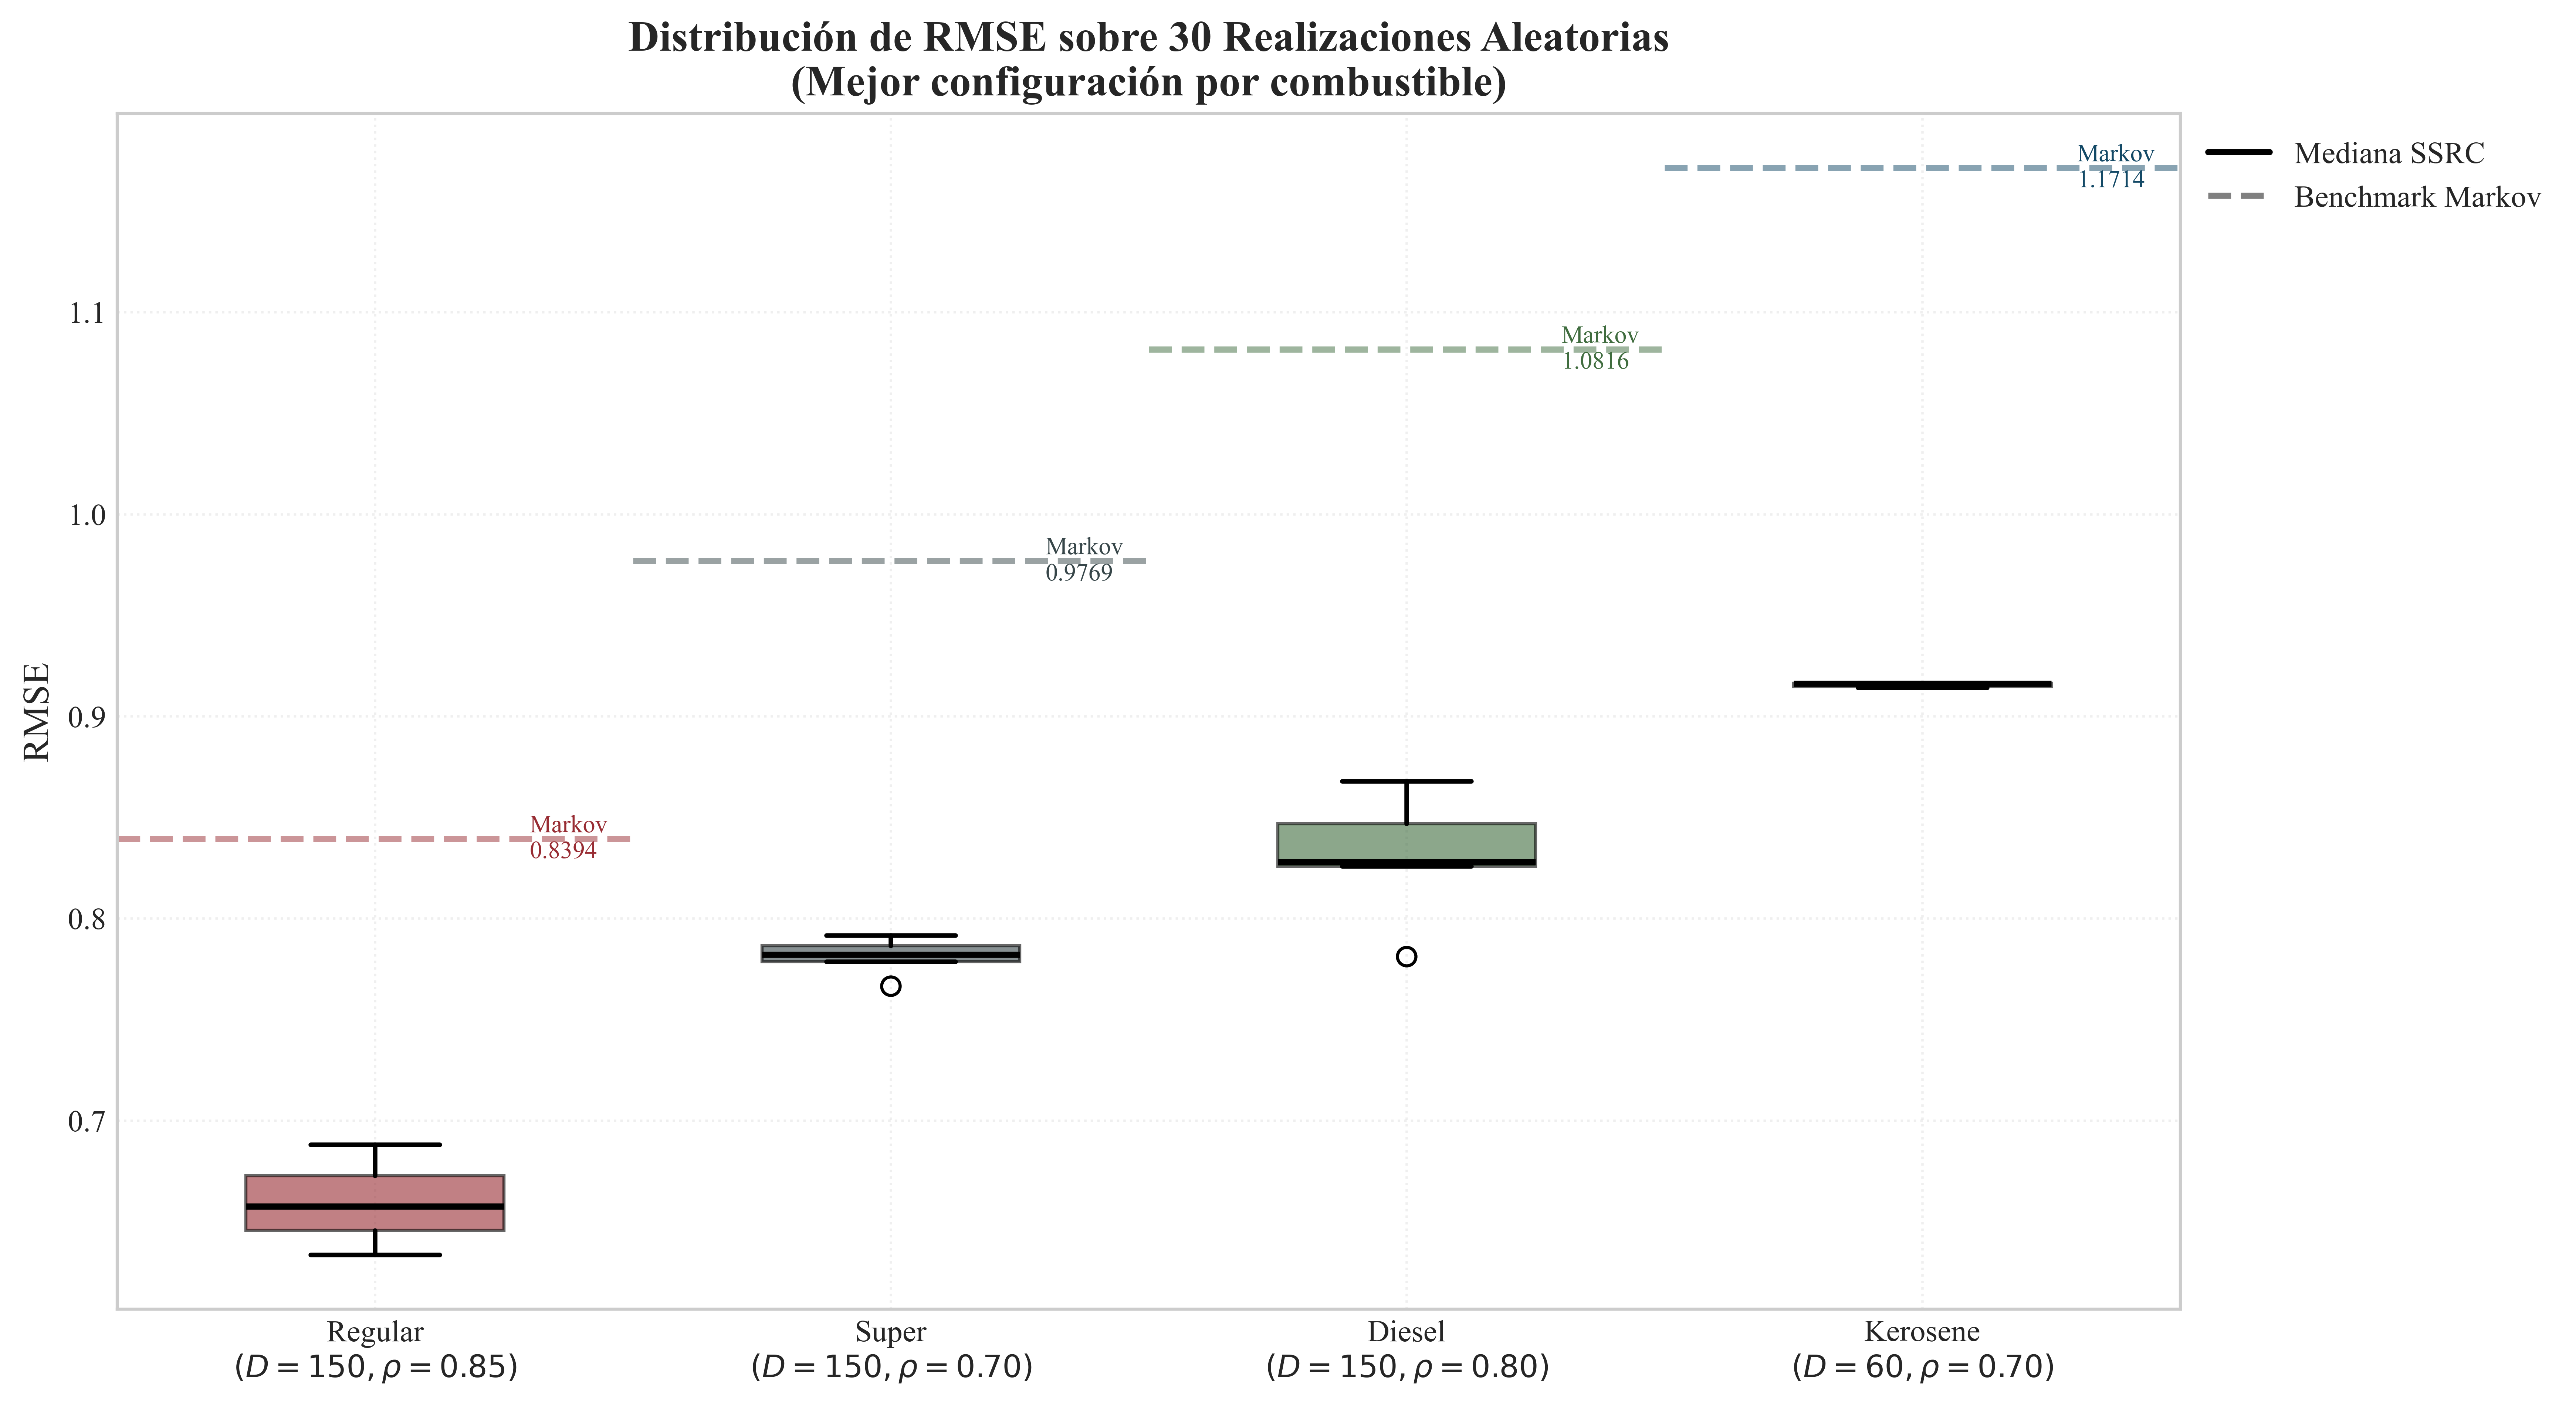
\includegraphics[width=0.95\textwidth]{figures/07_boxplot_realizations.png}
\caption{Distribución del RMSE del SSRC sobre 30 realizaciones.}
\label{fig:ssrc_boxplot}
\end{figure}

Como se observa en la Figura~\ref{fig:ssrc_boxplot}, se detalla la 
distribución del RMSE sobre 30 realizaciones aleatorias del SSRC bajo 
su mejor configuración. Las líneas horizontales punteadas representan 
el RMSE del benchmark Markoviano. Se destaca que en todas las series, 
la totalidad de las realizaciones produce un error inferior al benchmark. 
Las cajas estrechas indican una baja sensibilidad a la inicialización 
aleatoria de las matrices de entrada y de reservorio, con la mayor 
dispersión relativa observada en el combustible Regular.

La Figura~\ref{fig:ssrc_predictions} compara las predicciones
de ambos modelos contra los precios reales en el periodo fuera
de muestra.

\begin{figure}[H]
\centering
\includegraphics[width=1\textwidth]{figures/06_predictions_real_vs_models.png}
\caption{Comparación de pronósticos vs.\ precios reales.}
\label{fig:ssrc_predictions}
\end{figure}

En la Figura~\ref{fig:ssrc_predictions} se comparan los precios reales 
con los pronósticos de los modelos TCROC-Markov y TCROC-SSRC en el 
periodo fuera de muestra. Resulta visible que el modelo SSRC sigue 
con mayor precisión los puntos de inflexión del precio real, 
especialmente en los valles y las recuperaciones posteriores. 
Esta mejora es más evidente en las series de Diésel y Kerosene, 
donde el modelo Markoviano tiende a mostrar un sesgo de rezago más marcado.

% --- SUBSECCIÓN: Análisis de Sensibilidad y Estabilidad --- - - - - - - - - - - - - - - - - - - - - - - - - - - - - - -
\subsection{Análisis de Sensibilidad y Estabilidad}
\label{subsec:sensibilidad_hiperparametros}
% -------------------------------------------------------------------

La Figura~\ref{fig:ssrc_perturbation} evalúa empíricamente la cota
de perturbación de la Proposición~\ref{prop:acotacion_error}.

\begin{figure}[H]
\centering
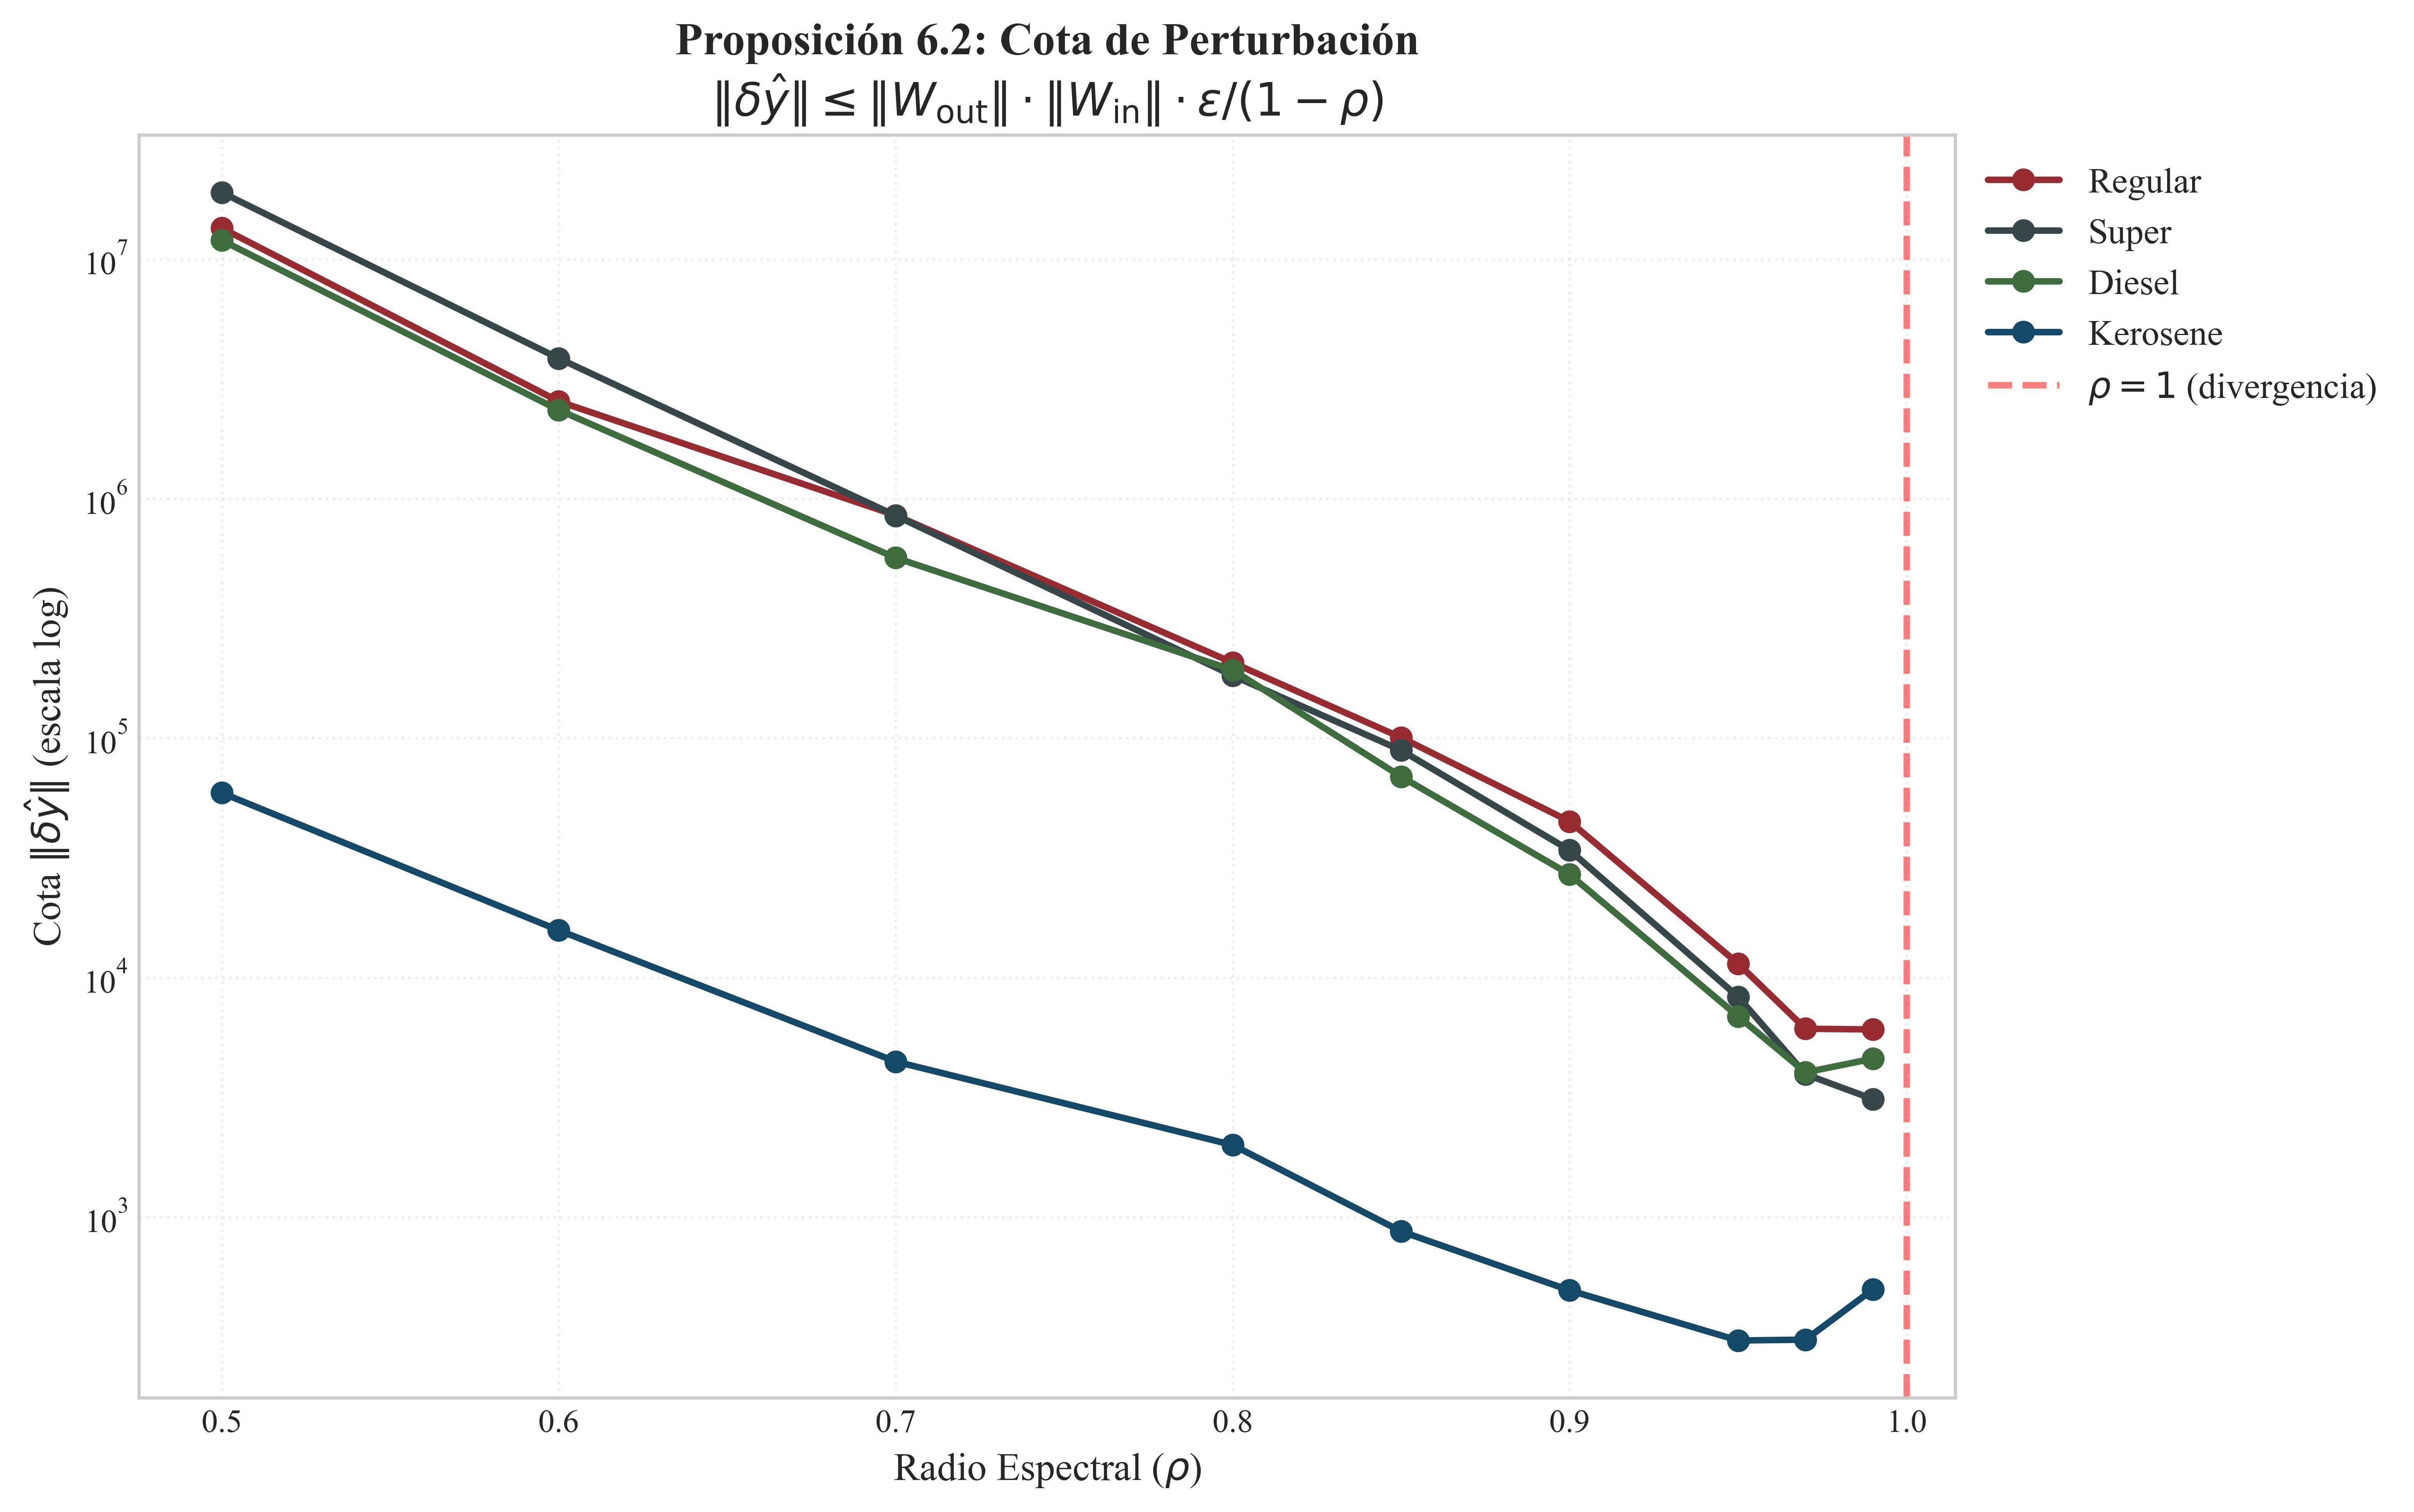
\includegraphics[width=0.95\textwidth]{figures/10_perturbation_bound.png}
\caption{Evaluación empírica de la cota de perturbación.}
\label{fig:ssrc_perturbation}
\end{figure}

La Figura~\ref{fig:ssrc_perturbation} evalúa empíricamente la cota de 
perturbación detallada en la Proposición~\ref{prop:acotacion_error} 
en función de $\rho$. La escala logarítmica muestra que las cotas 
teóricas son significativamente conservadoras comparadas con la 
variabilidad observada en la práctica. Se identifica que las cotas 
decrecen con el radio espectral debido a que la norma de los pesos de 
lectura disminuye más rápido de lo que aumenta el factor de memoria, 
resultando en estados más informativos que requieren pesos menores 
para el combustible Kerosene.

% --- SUBSECCIÓN: Representación de Regímenes en el Espacio del Reservorio --- - - - - - - - - - - - - - - - - - - - - - - - - - - - - - -
\subsection{Representación de Regímenes en el Espacio del Reservorio}
\label{subsec:regimenes_reservorio}
% -------------------------------------------------------------------

Una pregunta central es si la representación continua del reservorio
preserva la estructura de regímenes identificada por K-Means en el
capítulo anterior.  Las Figuras~\ref{fig:ssrc_states_pca},
\ref{fig:ssrc_scatter} y~\ref{fig:ssrc_price_regimes} abordan esta
cuestión desde tres perspectivas complementarias.

\begin{figure}[H]
\centering
\includegraphics[width=0.95\textwidth]{figures/05_reservoir_states_by_regime.png}
\caption{Proyección de los estados del reservorio mediante PCA.}
\label{fig:ssrc_states_pca}
\end{figure}

En la Figura~\ref{fig:ssrc_states_pca} se observa la proyección a dos 
dimensiones de los estados del reservorio $\vect{h}_t$ mediante PCA, 
con los puntos coloreados según los regímenes del capítulo anterior. 
Se evidencia que los regímenes forman clústeres geométricamente 
separados en el espacio latente del reservorio, a pesar de no contar 
con información explícita de clasificación. Las trayectorias suaves 
entre puntos indican que el reservorio mapea las transiciones entre 
regímenes como cambios continuos en lugar de saltos discretos.

\begin{figure}[H]
\centering
\includegraphics[width=0.95\textwidth]{figures/13_reservoir_regimes_scatter.png}
\caption{Relación entre retorno TCROC $\alpha_t$ y activación del reservorio.}
\label{fig:ssrc_scatter}
\end{figure}

La Figura~\ref{fig:ssrc_scatter} muestra la dispersión de $\alpha_t$ 
frente a la activación promedio del reservorio $\bar{h}_t$, diferenciada 
por regímenes. La relación monótona observada confirma que el reservorio 
preserva el orden dinámico de los regímenes: las activaciones negativas 
se vinculan a estados de caída, mientras que las positivas a estados de 
alza. La curvatura reflejada en series como Diésel evidencia la no 
linealidad de la función tangente hiperbólica utilizada.

\begin{figure}[H]
\centering
\includegraphics[width=0.95\textwidth]{figures/14_reservoir_price_regimes.png}
\caption{Identificación de regímenes de mercado mediante SSRC.}
\label{fig:ssrc_price_regimes}
\end{figure}

Finalmente, la Figura~\ref{fig:ssrc_price_regimes} presenta los regímenes 
identificados por el modelo SSRC superpuestos a la serie de precios original. 
La coincidencia entre las transiciones de color de fondo y los puntos de inflexión 
críticos del mercado, como la caída y recuperación durante el periodo de 2020, 
confirma que el marco TCROC-SSRC mantiene la interpretabilidad económica de los 
regímenes a pesar de procesar la información en un espacio de estados 
continuo de alta dimensión.

% --- SUBSECCIÓN: Discusión --- - - - - - - - - - - - - - - - - - - - - - - - - - - - - - -
\subsection{Discusión}
\label{subsec:ssrc_discusion}
% -------------------------------------------------------------------

Los resultados empíricos permiten responder a la pregunta central del
capítulo: ¿aporta la extensión no lineal una ganancia predictiva
sobre el modelo Markoviano lineal?

La respuesta es afirmativa y sustancial.  El SSRC reduce el RMSE
entre un 20\% y un 23\% en las cuatro series, con significancia
estadística confirmada por el test de Diebold-Mariano en tres de
cuatro casos.  Este resultado valida empíricamente la predicción del
Corolario~\ref{cor:jerarquia}: la generalización estrictamente más
expresiva del SSRC efectivamente captura estructura no lineal que el
modelo Markoviano no puede representar.

Tres hallazgos merecen interpretación detallada.  Primero, la
relevancia del factor de fuga $a$.  Los valores óptimos $a^* = 0.1$
para Regular y Diésel indican que la clave de la ganancia no es la
no linealidad per se, sino la \emph{memoria temporal adaptativa}:
el Leaky-ESN con $a = 0.1$ retiene el 90\% del estado previo,
actuando como un filtro de suavizado que complementa la ventana
$W \approx 50$ del operador TCROC.  En contraste, Kerosene con
$a^* = 1.0$ se beneficia de la memoria recurrente pura, consistente
con su dinámica más volátil y su mayor número de regímenes ($K = 5$).

Segundo, la saturación dimensional.  La
Figura~\ref{fig:ssrc_sens_D} muestra que la ganancia se satura
rápidamente: la diferencia entre $D = 20$ y $D = 150$ es inferior al
0.5\% en RMSE.  Esto indica que la complejidad no lineal intrínseca
del proceso generador de precios de combustibles hondureños es baja,
lo cual es consistente con un mercado regulado donde los ajustes
semanales son pequeños y predecibles.  El reservorio no necesita alta
dimensionalidad para capturar esta estructura.

Tercero, la robustez del ensemble.  La
Figura~\ref{fig:ssrc_boxplot} muestra que la totalidad de las 30
realizaciones produce RMSE inferior al benchmark Markoviano, con
rangos intercuartílicos estrechos.  Esto confirma que la ganancia no
es un artefacto de una inicialización afortunada, sino una propiedad
estructural del modelo.

Finalmente, cabe preguntarse qué estructura captura el reservorio que
el modelo Markoviano no puede representar.  La ganancia se atribuye a
la capacidad del SSRC de codificar \emph{asimetrías temporales} en la
dinámica de precios: las caídas y las recuperaciones no son simétricas
ni en magnitud ni en velocidad.  El modelo Markoviano, al operar sobre
estados discretos de un paso, trata las transiciones bajista$\to$estable
y alcista$\to$estable como eventos de naturaleza equivalente, gobernados
por probabilidades estáticas en $\hat{\mat{P}}$.  El reservorio, al
retener memoria continua de las últimas $\tau = 1/a$ semanas en su
vector de estado $\vect{h}_t$, puede distinguir la \emph{trayectoria}
que condujo al estado actual, y no únicamente el estado en sí mismo. Esta
capacidad es particularmente relevante para el pico de precios de
2022 y la recuperación posterior (visible en la
Figura~\ref{fig:ssrc_predictions}, semanas $\sim$5--20), donde el
SSRC anticipa mejor los puntos de inflexión que el modelo
Markoviano.

% --- SECCIÓN: Limitaciones ---
\section{Limitaciones}
\label{sec:ssrc_limitaciones}
% ===================================================================

\textbf{Sensibilidad a la inicialización.}  A diferencia del marco
TCROC-Markov, que es determinista dados los hiperparámetros, el SSRC
introduce variabilidad estocástica a través de las matrices aleatorias
$\mat{W}_{\text{in}}$ y $\mat{W}_{\text{res}}$.  Aunque la ESP
garantiza que la condición inicial $\vect{h}_0$ no afecta el
resultado, la \emph{elección} de las matrices de reservorio sí
influye en el desempeño.  El promediado sobre 30 realizaciones
(\textit{ensemble}) mitiga este efecto, como lo evidencia la baja
variabilidad observada en la Figura~\ref{fig:ssrc_boxplot}, pero
incrementa el costo computacional por un factor de 30.

\textbf{Condicionamiento numérico.}  Los números de condición
$\kappa(\mat{H}) \sim 10^{9}$--$10^{10}$ observados en la
Tabla~\ref{tab:verificaciones_teoricas} indican una sensibilidad
numérica potencialmente alta.  Aunque la estabilidad práctica está
asegurada por la regularización implícita del NNLS y el ensemble,
este condicionamiento impone un límite superior a la dimensión
útil del reservorio: aumentar $D$ más allá de $\sim$150 degradaría
$\kappa(\mat{H})$ sin ganancia predictiva.

\textbf{Interpretabilidad reducida.}  Los estados del reservorio
$\vect{h}_t \in \mathbb{R}^D$ carecen de la interpretación directa
que poseen los estados discretos $S_t \in \{s_1, \ldots, s_K\}$ del
modelo Markoviano.  No obstante, las
Figuras~\ref{fig:ssrc_states_pca}--\ref{fig:ssrc_price_regimes}
demuestran que la estructura de regímenes se preserva implícitamente
en el espacio del reservorio, lo que permite recuperar
interpretabilidad parcial mediante técnicas de reducción de
dimensionalidad.

\textbf{Selección de hiperparámetros del reservorio.}  Los parámetros
$(D, \rho_{\text{res}}, a)$ carecen de una teoría de selección
óptima análoga al AIC del modelo Markoviano.  La búsqueda en grilla de 240 configuraciones iterativas es computacionalmente costosa; la incorporación de metaheurísticas como la Optimización Bayesiana (Gaussian Processes) se vuelve fundamental. Además, aunque K-Means es estadísticamente viable, la discretización univariada permite la instanciación de algoritmos de partición dinámica formal continua como el modelo puro unidimensional de Fisher-Jenks para alcanzar los verdaderos óptimos probados y globales de manera robusta y exacta.

\textbf{Conservadurismo de la cota de perturbación.}  La
Proposición~\ref{prop:acotacion_error} proporciona una cota en el
peor caso que, como se evidencia en la
Figura~\ref{fig:ssrc_perturbation}, sobreestima la inestabilidad
real por varios órdenes de magnitud.  Una cota más ajustada
requeriría análisis probabilístico que incorpore la distribución de
$\alpha_t$ y la estructura de $\mat{W}_{\text{res}}$, lo cual
constituye un desafío de interés dentro del trabajo futuro; las metodologías análogas de normas afines y principalmente la aplicación del Teorema del Círculo de Gerschgorin sobre la matriz dispersa $\mat{W}_{\text{res}}$ posibilitarían una envolvente teórica significativamente más ajustada que la hipótesis conservadora basal propuesta.

% --- SECCIÓN: Conclusiones ---
\section{Conclusiones}
\label{sec:ssrc_conclusiones}
% ===================================================================

Este capítulo ha establecido la relación formal entre el marco
TCROC-Markov desarrollado a lo largo de la tesis y la computación
de reservorio no lineal.  Los resultados principales son:

\textbf{Sobre la conexión teórica.}  Se demostró
(Teorema~\ref{teo:inclusion}) que TCROC-Markov es un caso particular
del SSRC, obtenido al fijar $\mat{W}_{\text{res}} = \mat{0}$,
$\sigma = \mathrm{id}$ y $a = 1$.  Esta relación de inclusión
establece una \textbf{jerarquía de modelos}: TCROC-Markov (lineal,
interpretable, estados discretos) $\subset$ TCROC-SSRC (no lineal,
aproximador universal, estados continuos).  El
Corolario~\ref{cor:jerarquia} garantiza que la extensión es
estrictamente más expresiva, y la verificación numérica
(Figura~\ref{fig:ssrc_inclusion}) confirma la identidad a nivel de
precisión de máquina.

\textbf{Sobre la estimación.}  La capa de lectura del SSRC se estima
mediante el mismo procedimiento NNLS de los capítulos anteriores.
El Teorema~\ref{teo:existencia_wout} establece que las propiedades
de existencia y unicidad se heredan directamente.  La restricción
de no negatividad, además de preservar la interpretación como
combinación positiva de filtros, aporta regularización implícita que
mitiga el condicionamiento numérico adverso ($\kappa \sim 10^{9}$).

\textbf{Sobre el factor de fuga.}  La variante Leaky-ESN
(Definición~\ref{def:leaky_esn}) con $a < 1$ resultó esencial para
tres de cuatro series, indicando que la principal ganancia del SSRC
sobre TCROC-Markov reside en la \emph{memoria temporal adaptativa}
más que en la no linealidad pura.  Los valores $a^* = 0.1$ para
Regular y Diésel implican una constante de tiempo efectiva de
$\tau = 10$ semanas, complementaria a la ventana TCROC de 50--52
semanas.

\textbf{Sobre la aplicación empírica.}  El SSRC reduce el RMSE entre
un 20\% y un 23\% respecto al modelo Markoviano, con significancia
estadística confirmada por el test de Diebold-Mariano para Súper
($p = 0.002$), Diésel ($p = 0.033$) y Kerosene ($p = 0.006$).  La
totalidad de las 30 realizaciones aleatorias produce RMSE inferior al
benchmark Markoviano, y la estructura de regímenes económicos se
preserva en el espacio latente del reservorio.

\textbf{Perspectiva.}  La arquitectura TCROC-SSRC aquí desarrollada
establece que el paradigma de reservorio aporta ganancia predictiva
en mercados de combustibles regulados, a costa de interpretabilidad.
La extensión natural es hacia sistemas multivariados y acoplados,
donde la capacidad de aproximación no lineal del reservorio puede
explotarse más plenamente en contextos con mayor riqueza estructural.

% ===================================================================
% CAPÍTULO: Conclusiones Generales y Trabajo Futuro
